\chapter{Experiments and Evaluation}
\section{Experimental Setup}
\par All experiments in this chapter are built on the unified pipeline
described in Chapter 3. The input images are first processed by size
normalization and grayscale conversion, and then divided into non-overlapping
patches of fixed size. Unless otherwise stated, all experiments use a patch
size of $32\times32$. The labels are generated by the automatic labeling rules
based on Laplacian, Sobel, and FFT \cite{5739529,1284395}, and are organized
into a binary classification task (both the sharp threshold and the blur
threshold are set to $0.75$) and a three-class classification task (the sharp
threshold is set to $0.75$ and the blur threshold is set to $0.4$),
respectively. In both training and validation, textureless samples ($y=-1$)
are filtered out, and only samples whose focus state can be judged stably are
retained for comparison.

\par In terms of data scale, the experiments in this thesis use a total of
$350$ original images, among which the validation set contains $75$ images and
the remaining images are used for training. After size normalization, all
images are divided into non-overlapping $32\times32$ patches. Since the
original resolutions are different, each image usually generates about
$2000\sim3000$ patches, and therefore the final training and validation are
performed on a large patch-level sample set. It should be noted that although
the number of patches is much larger than the number of original images, these
patches are not independently collected samples, but are obtained by splitting
a limited number of original images. Therefore, when reporting patch-level
experimental results, this thesis still keeps the number of original images as
an explanation of the data scale.

\par To ensure comparability among different methods, the classical machine
learning models and the CNN use the same training/validation split. The
classical models include decision tree, random forest, and support vector
machine based on Nystr\"{o}m kernel approximation. Their input is the
normalized grayscale patch vector, and PCA dimensionality reduction is
uniformly applied according to the pre-experimental results
\cite{perry2025inference,zheng2021application}. The CNN directly takes the
single-channel patch as input and uses a unified lightweight architecture and
number of training epochs. For the class imbalance problem, the classical
models use class weights, while the CNN uses loss weights calculated from
class frequency by default, and further compares whether weighted sampling is
introduced in the supplementary experiment.

\par In the experimental organization, this chapter first determines the PCA
retention ratio and the number of CNN training epochs through pre-experiments,
then conducts the main experiments under unified parameters, and further
combines a scan over different training sample ratios to analyze the influence
of training sample size on different models. In addition to performance
metrics, training time is also recorded, so that the applicability of
different methods in patch-based image focus detection can be evaluated from
both recognition effect and computational cost.

\section{Evaluation Metrics and Prediction Settings}
\par This thesis focuses on the recognition ability of local sharp regions, and
the sharp class (sharp, label $1$) is usually the minority class in the
dataset. Therefore, using overall accuracy alone is not sufficient for model
evaluation. By comparison, precision, recall, F1-score, and macro F1
\cite{schutze2008introduction} can better reflect the discrimination quality
of the model for each class, especially for sharp regions. Among them, recall
measures the proportion of real sharp regions that are successfully detected,
precision measures the proportion of regions predicted as sharp that truly
belong to the sharp class, F1-score is used to evaluate precision and recall
jointly, and macro F1 takes the equally weighted average of the F1-scores of
all classes. Therefore, it is more suitable for cases with imbalanced class
distribution.

\par In addition to classification performance, training time is also treated as
an important evaluation dimension in this thesis. If one parameter setting
brings only limited performance gain but significantly increases training cost,
it is not favorable for the unified execution of subsequent experiments or the
reproducibility of results. Therefore, the pre-experimental stage always makes
judgment by combining performance metrics and computational cost, and on this
basis determines the unified parameters used in the formal experiments.

\section{Pre-Experiments for Parameter Selection}
\subsection{PCA Parameter Selection}
\par The feature dimension of a flattened original patch is $1024$. If it is
directly fed into classical classifiers, the training cost becomes high and
more redundant information may also be introduced. Therefore, this thesis first
determines the PCA parameter used in the subsequent experiments through
comparative experiments. Specifically, under both the three-class and binary
task settings, the same decision tree, random forest, and Nystr\"{o}m-SVM
configurations are used to compare PCA retention ratios
\(\in\{0.95,0.99,0.995,0.999\}\). The analysis in this section jointly
considers precision, recall, F1-score, macro F1, and training time on the
validation set, with particular attention to recall and F1-score of the sharp
class.

\par\medskip \noindent\textbf{Three-Class Setting.} \par The experimental
results for the three-class task are shown in
Table~\ref{tab:pca-triclass-pca}. The table lists the sharp-class precision,
recall, F1, macro F1, and training time of the three models under different
PCA retention ratios, so as to compare the performance and cost of different
parameter settings in a comprehensive way.

\begin{table}[htbp]
    \centering
    \caption{Comprehensive comparison under different PCA retention ratios in the three-class task}
    \label{tab:pca-triclass-pca}
    \begin{tabular}{llccccc}
        \toprule
        PCA & Model & Precision$_{\mathrm{focus}}$ & Recall$_{\mathrm{focus}}$ &
        F1$_{\mathrm{focus}}$ & Macro F1 & Time (s) \\
        \midrule
        0.95  & Decision Tree & 0.26 & 0.60 & 0.36 & 0.57 & 5.53   \\
        0.95  & Random Forest & 0.32 & 0.49 & 0.38 & 0.62 & 25.53  \\
        0.95  & SVM           & 0.41 & 0.21 & 0.28 & 0.60 & 353.66 \\
        0.99  & Decision Tree & 0.55 & 0.81 & 0.65 & 0.78 & 45.43  \\
        0.99  & Random Forest & 0.69 & 0.82 & 0.75 & 0.85 & 82.96  \\
        0.99  & SVM           & 0.64 & 0.74 & 0.69 & 0.83 & 115.49 \\
        0.995 & Decision Tree & 0.65 & 0.83 & 0.73 & 0.82 & 99.17  \\
        0.995 & Random Forest & 0.75 & 0.91 & 0.83 & 0.88 & 116.74 \\
        0.995 & SVM           & 0.76 & 0.86 & 0.81 & 0.89 & 93.24  \\
        0.999 & Decision Tree & 0.71 & 0.86 & 0.78 & 0.85 & 349.45 \\
        0.999 & Random Forest & 0.84 & 0.94 & 0.88 & 0.90 & 223.02 \\
        0.999 & SVM           & 0.88 & 0.97 & 0.92 & 0.89 & 83.07  \\
        \bottomrule
    \end{tabular}
\end{table}

\par Under the three-class setting, when the PCA retention ratio is $0.95$, the
overall performance of all three models is relatively weak, which indicates
that excessive dimensionality reduction weakens local discriminative
information related to focus state. As the retention ratio increases, the
recall, F1-score, and macro F1 of each model all improve significantly. A
comprehensive comparison shows that when the retention ratio is $0.995$, the
three models already achieve a relatively good balance between sharp-class
recognition ability and overall class balance, and the macro F1 of random
forest and SVM reaches $0.88$ and $0.89$, respectively. By comparison,
although $0.999$ further improves sharp-class recall and F1 in some models,
its gain is not consistent across models, and the training time of decision
tree and random forest increases significantly. Therefore, for the three-class
task, a PCA retention ratio of $0.995$ shows a more stable balance between
performance and computational cost.

\par\medskip \noindent\textbf{Binary Setting.} \par The experimental results
for the binary task are shown in Table~\ref{tab:pca-binary-pca}. Similar to the
three-class case, the table gives the sharp-class precision, recall, F1,
macro F1, and training time of the three models under different PCA retention
ratios.

\begin{table}[htbp]
    \centering
    \caption{Comprehensive comparison under different PCA retention ratios in the binary task}
    \label{tab:pca-binary-pca}
    \begin{tabular}{llccccc}
        \toprule
        PCA & Model & Precision$_{\mathrm{focus}}$ & Recall$_{\mathrm{focus}}$ &
        F1$_{\mathrm{focus}}$ & Macro F1 & Time (s) \\
        \midrule
        0.95  & Decision Tree & 0.23 & 0.78 & 0.35 & 0.58 & 5.37   \\
        0.95  & Random Forest & 0.27 & 0.73 & 0.40 & 0.62 & 26.34  \\
        0.95  & SVM           & 0.25 & 0.76 & 0.37 & 0.60 & 122.06 \\
        0.99  & Decision Tree & 0.48 & 0.88 & 0.62 & 0.78 & 47.49  \\
        0.99  & Random Forest & 0.56 & 0.92 & 0.70 & 0.82 & 95.94  \\
        0.99  & SVM           & 0.49 & 0.94 & 0.64 & 0.79 & 40.93  \\
        0.995 & Decision Tree & 0.59 & 0.90 & 0.71 & 0.83 & 104.46 \\
        0.995 & Random Forest & 0.66 & 0.96 & 0.78 & 0.87 & 129.81 \\
        0.995 & SVM           & 0.60 & 0.97 & 0.74 & 0.85 & 18.42  \\
        0.999 & Decision Tree & 0.65 & 0.89 & 0.75 & 0.86 & 371.16 \\
        0.999 & Random Forest & 0.73 & 0.98 & 0.83 & 0.91 & 260.94 \\
        0.999 & SVM           & 0.81 & 0.99 & 0.89 & 0.94 & 9.46   \\
        \bottomrule
    \end{tabular}
\end{table}

\par Under the binary setting, as the PCA retention ratio increases, the recall
and F1-score of each model on the sharp class continue to improve. Among them,
when the retention ratio is $0.999$, the precision, recall, and F1-score of
the SVM on the sharp class reach $0.81$, $0.99$, and $0.89$, respectively, and
the macro F1 reaches $0.94$, which is the best result in this group. Random
forest also shows relatively good sharp-class recall and F1-score under this
setting. However, compared with $0.995$, the advantage of $0.999$ is mainly
reflected in the binary task and does not show consistent improvement in the
three-class task. At the same time, a higher PCA retention ratio also
corresponds to greater training cost. For example, the training times of
decision tree and random forest at $0.999$ are both much higher than those at
$0.995$.

\par By jointly considering the results of the three-class and binary tasks,
this thesis finally selects a PCA retention ratio of $0.995$ as the unified
PCA parameter for the subsequent experiments. The reason is that this setting
maintains a relatively high level on recall, F1-score, and macro F1 in the
three-class task, while also keeping good performance in the binary task. It
should be noted that $0.999$ can indeed achieve higher results on the sharp-
class recall, F1-score, and some macro F1 values in some models, especially in
individual settings. However, this advantage does not appear consistently
across the binary and three-class tasks or across different models. At the
same time, compared with $0.999$, the overall training cost of $0.995$ is
lower. Therefore, the parameter selection in this thesis is not based on local
optimum from a single experiment, but places more emphasis on cross-task
consistency, training cost, and reproducibility. Based on a comprehensive
consideration of performance and computational cost, the PCA retention ratio
$0.995$ is selected as the unified parameter for the subsequent experiments.

\subsection{Epoch Parameter Selection}
\par After determining the PCA parameter used by the classical models, this
thesis further performs pre-experiments on the number of CNN training epochs to
determine the unified epoch number used in the subsequent main experiments.
Specifically, under the three-class setting (sharp threshold $0.75$, blur
threshold $0.4$) and the binary setting (both sharp and blur thresholds set to
$0.75$), the influence of the training epochs
\(\in\{10,20,30,50,60\}\) on validation performance and training time is
compared. Since this thesis focuses on the detection ability of sharp regions,
the analysis still mainly considers precision, recall, F1-score, and macro F1
of the sharp class (sharp, label $1$), together with training time and the
decreasing trend of loss.

\par\medskip \noindent\textbf{Three-Class Setting.} \par The experimental
results of different epoch numbers in the three-class task are shown in
Table~\ref{tab:epoch-triclass-cnn}. The table lists the precision, recall, F1,
macro F1, and training time of the sharp class, so as to observe the changes
in performance and cost as the number of training epochs increases.

\begin{table}[htbp]
    \centering
    \caption{Comprehensive comparison of CNN under different epochs in the three-class task}
    \label{tab:epoch-triclass-cnn}
    \begin{tabular}{cccccc}
        \toprule
        Epoch & Precision$_{\mathrm{focus}}$ & Recall$_{\mathrm{focus}}$ &
        F1$_{\mathrm{focus}}$ & Macro F1 & Time (s) \\
        \midrule
        10 & 1.00 & 0.65 & 0.79 & 0.81 & 245.25  \\
        20 & 1.00 & 0.71 & 0.83 & 0.84 & 506.76  \\
        30 & 1.00 & 0.60 & 0.75 & 0.83 & 758.34  \\
        50 & 1.00 & 0.63 & 0.77 & 0.85 & 1254.64 \\
        60 & 1.00 & 0.69 & 0.81 & 0.86 & 1504.51 \\
        \bottomrule
    \end{tabular}
\end{table}

\par From the training process, the loss decreases most clearly within the
first $20$ epochs, from $1269.50$ to $521.27$. When the training continues to
$30$ epochs, it further decreases to $500.73$, which indicates that the model
is still in a continuous convergence stage. After that, although the loss
continues to decrease, fluctuations start to increase, and it only further
drops to $478.99$ at $60$ epochs. In terms of validation results, at $20$
epochs the sharp-class recall and F1-score reach $0.71$ and $0.83$,
respectively, which is a clear improvement over $10$ epochs. At $30$ epochs,
although the sharp-class recall drops to $0.60$, the overall accuracy rises to
$0.8709$, indicating that the overall discrimination ability of the model is
still improving. By comparison, although $50$ and $60$ epochs bring a slight
improvement in macro F1, the training time increases to $1254.64$s and
$1504.51$s, respectively, and the computational cost grows significantly.
Therefore, for the three-class task, $30$ epochs can still push the model to
continue converging while keeping the training cost at a relatively acceptable
level.

\par\medskip \noindent\textbf{Binary Setting.} \par The experimental results of
different epoch numbers in the binary task are shown in
Table~\ref{tab:epoch-binary-cnn}. Similar to the three-class task, the table
gives the sharp-class precision, recall, F1, macro F1, and training time.

\begin{table}[htbp]
    \centering
    \caption{Comprehensive comparison of CNN under different epochs in the binary task}
    \label{tab:epoch-binary-cnn}
    \begin{tabular}{cccccc}
        \toprule
        Epoch & Precision$_{\mathrm{focus}}$ & Recall$_{\mathrm{focus}}$ &
        F1$_{\mathrm{focus}}$ & Macro F1 & Time (s) \\
        \midrule
        10 & 1.00 & 0.68 & 0.81 & 0.89 & 235.81  \\
        20 & 1.00 & 0.71 & 0.83 & 0.91 & 468.89  \\
        30 & 0.99 & 0.73 & 0.84 & 0.91 & 686.42  \\
        50 & 1.00 & 0.67 & 0.81 & 0.89 & 1140.89 \\
        60 & 1.00 & 0.72 & 0.84 & 0.91 & 1366.49 \\
        \bottomrule
    \end{tabular}
\end{table}

\par Under the binary setting, the loss is also concentrated in the first $20$
epochs, rapidly decreasing from $553.42$ to $174.09$. At $30$ epochs, it
further decreases to $162.95$, while when training continues to $60$ epochs,
it only further decreases to $147.87$. From the validation results, $20$
epochs already raises the sharp-class F1-score to $0.83$ and the macro F1 to
$0.91$. At $30$ epochs, the recall further increases to $0.73$ and the
F1-score further rises to $0.84$, which indicates that the model can still
obtain some gain at this stage. By comparison, the recall and F1-score at $50$
epochs instead decline, while the results at $60$ epochs are close to those at
$30$ epochs but require much longer training time. This shows that the
marginal benefit of continuing to increase the number of training epochs is
already weak.

\par By jointly considering the results of the three-class and binary tasks,
this thesis finally selects $30$ epochs as the unified training epoch number
for the subsequent CNN experiments. The selection criterion here is not only
the local optimum of the sharp-class F1-score in a single task, but also
considers cross-task consistency, sufficient convergence, and training cost.
Compared with $20$ epochs, $30$ epochs can continue to push loss convergence
without allowing training time to further worsen to the level of $50$ or $60$
epochs, and can also bring higher sharp-class recall and F1-score in the
binary task. For the three-class task, although $20$ epochs is higher on
sharp-class recall and F1-score, $30$ epochs reflects a more sufficient
training process and is therefore more suitable as the unified parameter for
the subsequent main experiments. Based on this consideration that unified
parameters are preferred over local optimum of a single metric, this thesis
sets $30$ training epochs as the unified parameter for the subsequent
experiments.

\section{Main Experiments}
\par After completing the pre-experiments for PCA and epochs, this thesis
conducts the main experiments under a unified configuration. Specifically, the
classical models all use a PCA retention ratio of $0.995$, the CNN is
uniformly trained for $30$ epochs, and the patch size is fixed at
$32\times 32$. At the same time, to observe the influence of data scale on
model performance, a full scan over training sample ratios
\(\{20,40,60,80,100\}\%\) is performed under both the binary setting (both
sharp and blur thresholds are set to $0.75$) and the three-class setting
(sharp threshold $0.75$, blur threshold $0.4$). The preprocessing time is
$475.38$s for the binary experiment and $550.00$s for the three-class
experiment, which indicates that the three-class label partition brings higher
data preparation cost. The following analysis first compares the final results
under $100\%$ training samples, and then combines the full log to analyze the
behavior of different models as training scale changes.

\par\medskip \noindent\textbf{Binary Setting.} \par In the binary task, the
validation set contains $121405$ blur patches and $14665$ sharp patches, and
the class imbalance is obvious. Therefore, this thesis focuses on the
precision, recall, and F1-score of the sharp class (sharp, label $1$), and
uses macro F1 as an auxiliary indicator of overall class balance.
Table~\ref{tab:main-binary-100} gives the main experimental results of the four
models under $100\%$ training samples.

\begin{table}[htbp]
    \centering
    \caption{Main experimental results under $100\%$ training samples in the binary task}
    \label{tab:main-binary-100}
    \begin{tabular}{lcccccc}
        \toprule
        Model & Accuracy & Precision$_{\mathrm{focus}}$ &
        Recall$_{\mathrm{focus}}$ & F1$_{\mathrm{focus}}$ & Macro F1 & Time (s)
        \\
        \midrule
        Decision Tree & 0.9223 & 0.59 & 0.90 & 0.71 & 0.83 & 103.48 \\
        Random Forest & 0.9413 & 0.66 & 0.96 & 0.78 & 0.87 & 120.80 \\
        SVM           & 0.9268 & 0.60 & 0.97 & 0.74 & 0.85 & 17.68  \\
        CNN           & 0.9709 & 0.99 & 0.73 & 0.84 & 0.91 & 684.51 \\
        \bottomrule
    \end{tabular}
\end{table}

\begin{figure}[htbp]
    \centering
    \begin{subfigure}{0.47\textwidth}
        \centering
        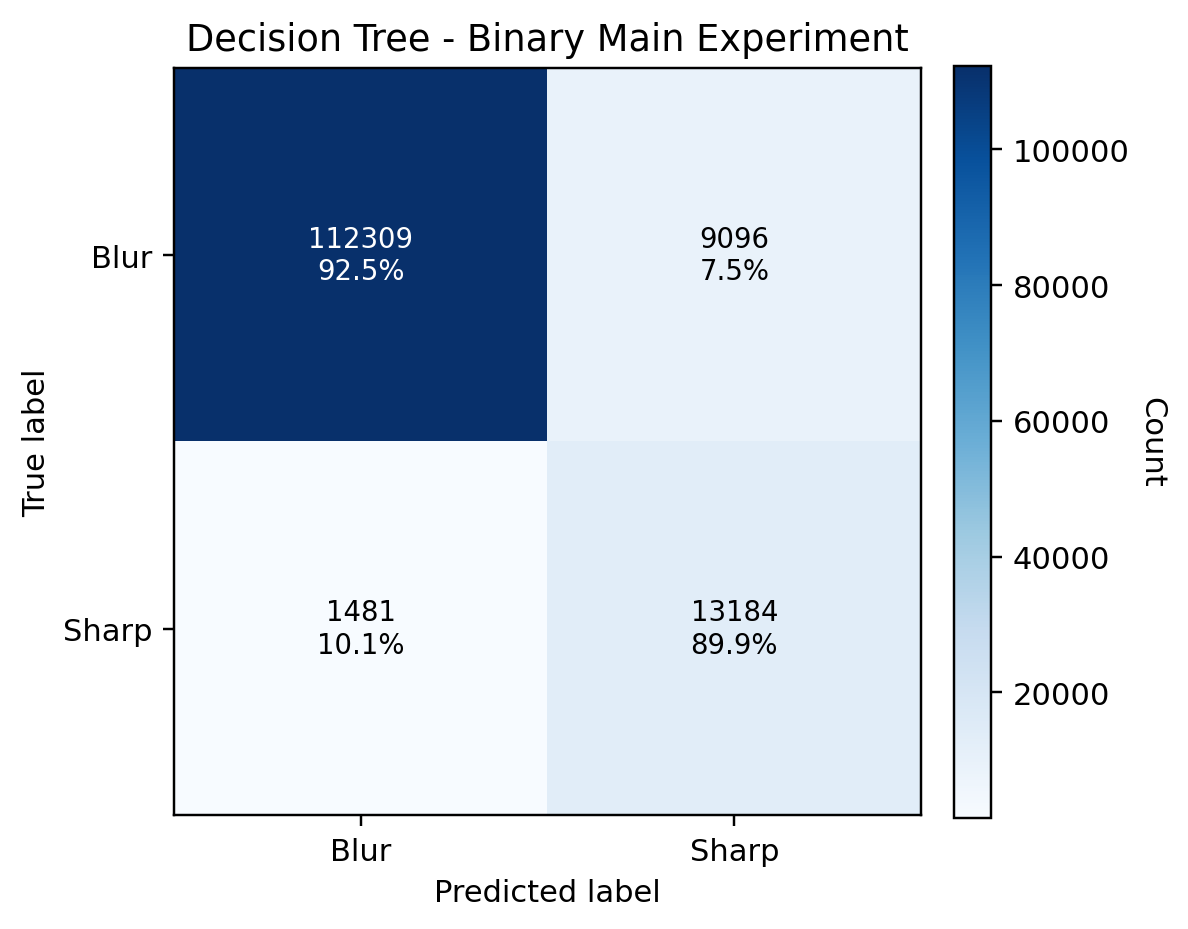
\includegraphics[width=\linewidth]{images/cm_main_2c_decision_tree.png}
        \caption{Decision Tree}
    \end{subfigure}
    \hfill
    \begin{subfigure}{0.47\textwidth}
        \centering
        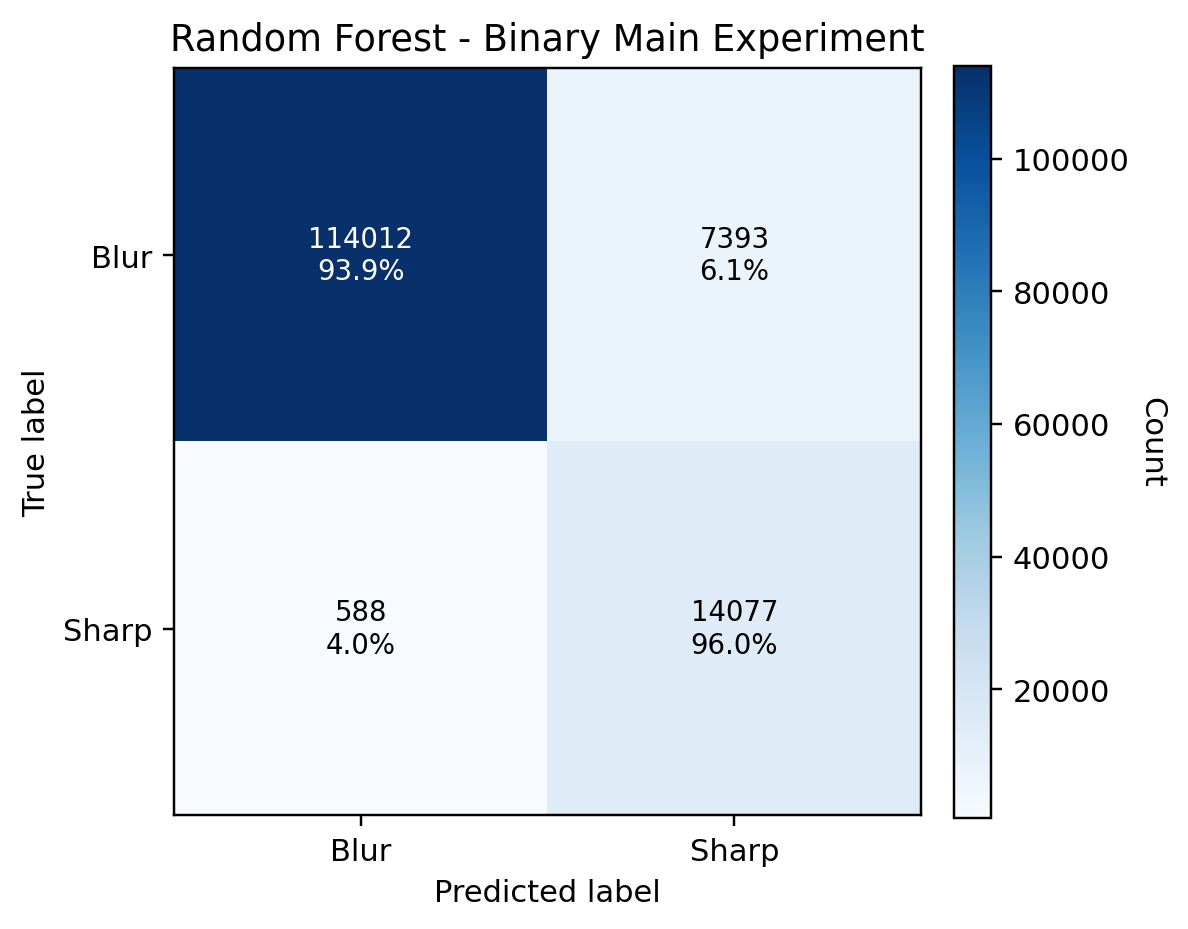
\includegraphics[width=\linewidth]{images/cm_main_2c_random_forest.png}
        \caption{Random Forest}
    \end{subfigure}

    \vspace{0.6em}

    \begin{subfigure}{0.47\textwidth}
        \centering
        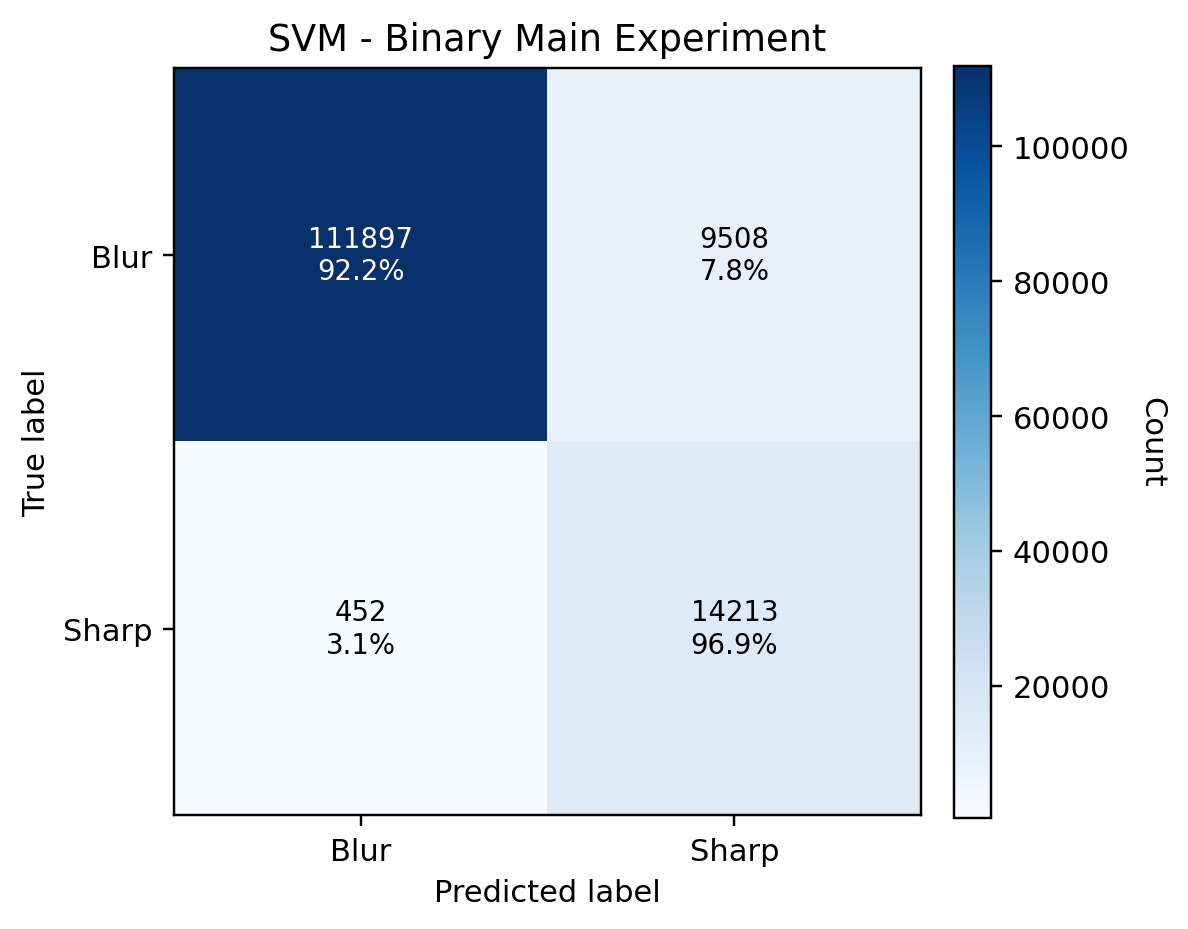
\includegraphics[width=\linewidth]{images/cm_main_2c_svm.png}
        \caption{SVM}
    \end{subfigure}
    \hfill
    \begin{subfigure}{0.47\textwidth}
        \centering
        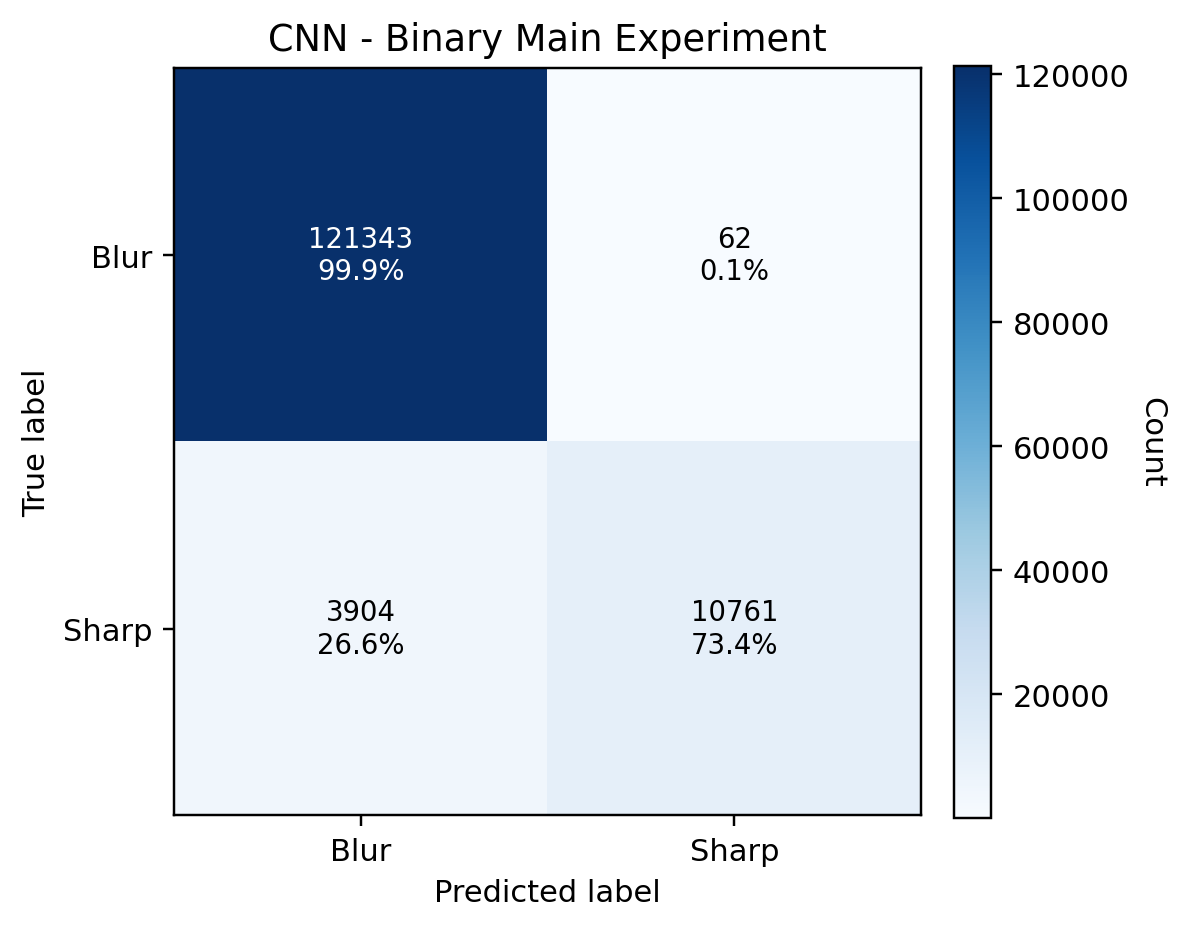
\includegraphics[width=\linewidth]{images/cm_main_2c_cnn.png}
        \caption{CNN}
    \end{subfigure}
    \caption{Confusion matrices of the four models under $100\%$ training samples in the main binary experiment}
    \label{fig:cm-main-2c}
\end{figure}

\par From the final results, the CNN obtains the highest sharp-class F1-score
($0.84$) and the highest macro F1 ($0.91$) in the binary task. Therefore, if
the main criterion is the overall recognition quality of sharp regions, it is
the best model under this setting. Its advantage mainly comes from extremely
high precision ($0.99$), which indicates that the model is very conservative
when judging sharp regions and almost never misclassifies blurred patches as
sharp. At the same time, however, the recall is $0.73$, which means that some
real sharp regions are still missed. By comparison, the sharp-class F1-score
of the SVM is $0.74$, which is lower than that of the CNN, but its recall
reaches $0.97$, the highest among the four models. This indicates that it is
more inclined to ensure that sharp regions are not missed, although this
strategy introduces more false positives, thus lowering precision and making it
difficult for F1-score to increase further. Random forest provides a compromise
between the two. Its sharp-class recall is $0.96$ and its F1-score is $0.78$.
Its overall performance is clearly better than that of the decision tree, but
it is still lower than that of the CNN. From the perspective of training time,
this performance difference is accompanied by a large computational cost. Under
$100\%$ samples, the CNN needs $684.51$s, while the SVM only requires
$17.68$s, random forest requires $120.80$s, and decision tree requires
$103.48$s. In other words, although the CNN is the best model on F1-score, its
cost is about $39$ times that of the SVM. Therefore, if later experimental
iteration, parameter search, or deployment efficiency is considered, time cost
must be evaluated together with the performance result.

\par Figure~\ref{fig:cm-main-2c} gives the confusion matrices of the four
models in the main binary experiment under $100\%$ training samples
\cite{schutze2008introduction}. Overall, the four models can all distinguish
the blur class and the sharp class relatively well, but they show clear
differences in the distribution of false positives and false negatives. The CNN
has the fewest off-diagonal items, especially very few errors in the direction
of ``blur $\rightarrow$ sharp''. The SVM and random forest show stronger
sharp-class detection ability, but this is accompanied by more cases where blur
patches are misclassified as sharp. The decision tree shows relatively higher
errors in both directions, and therefore performs worse overall than the other
three models.

\par From the detailed structure of the confusion matrices, the advantage of the
CNN mainly lies in its extremely small number of false positives: only $62$
blur patches are misclassified as sharp, while the numbers for decision tree,
random forest, and SVM are $9096$, $7393$, and $9508$, respectively. This
shows that the CNN is very conservative when identifying sharp regions and can
therefore achieve a sharp-class precision close to $1.00$. However, this
conservative strategy also leads to many misses. It classifies $3904$ real
sharp patches as blur, which is clearly higher than random forest's $588$ and
SVM's $452$, and this limits recall. In contrast, the confusion matrices of
the SVM and random forest reflect another strategy: they improve sharp-class
recall by significantly reducing false negatives, but the cost is more false
positives, so precision decreases. The decision tree fails to achieve an
effective balance between the two, which indicates that its ability to express
class boundaries in the current task is relatively limited.

\par By combining the full scan results from $20\%$ to $100\%$ samples, it can
be seen that different models have clearly different sensitivity to sample
size. The sharp-class F1-score of the decision tree only slowly increases from
$0.69$ to $0.71$, and macro F1 only rises from $0.82$ to $0.83$, which
indicates that the gain from additional samples is limited. Random forest shows
a more obvious precision-recall trade-off: as the training ratio increases
from $20\%$ to $100\%$, the sharp-class recall rises continuously from $0.84$
to $0.96$, but precision drops from $0.79$ to $0.66$, which instead makes the
sharp-class F1-score decline from $0.81$ to $0.78$. This shows that more
training data make random forest predict the sharp class more aggressively,
thus reducing missed detections but also increasing false detections. The SVM
shows the most stable results: in all five training ratios, its sharp-class
recall always remains at $0.97$, its F1-score stays around $0.74$, and its
training time only increases from $3.64$s to $17.68$s. It is therefore the
lowest-cost traditional method and also the most stable on recall. The CNN is
the most sensitive to data scale. Under $20\%$, $40\%$, and $80\%$ samples,
its sharp-class recall is only $0.69$, $0.67$, and $0.68$, respectively, but
its sharp-class F1-score already reaches $0.81$, $0.80$, and $0.81$, and then
further improves to $0.84$ at $100\%$ samples. This indicates that deep models
depend more on sufficient samples to learn stable local sharpness patterns.
When training data are insufficient, their high-precision advantage cannot be
fully converted into higher recall, but as the number of samples increases,
the F1-score can still continue to benefit.

\par Therefore, in the binary task, if the goal is to obtain the highest
overall sharp-class F1-score together with a relatively good macro F1, the CNN
is the best choice. If the goal is to detect sharp regions as completely as
possible while controlling training cost, the SVM is a more cost-effective
option. If a balance between F1 and time is preferred, random forest is also an
acceptable intermediate solution.

\par\medskip \noindent\textbf{Three-Class Setting.} \par In the three-class
task, patches are divided into blur, sharp, and intermediate classes. The
validation set contains $65830$, $14665$, and $55575$ samples, respectively,
and the sharp class (label $1$) is still the minority class.
Table~\ref{tab:main-triclass-100} gives the main experimental results under
$100\%$ training samples.

\begin{table}[htbp]
    \centering
    \caption{Main experimental results under $100\%$ training samples in the three-class task}
    \label{tab:main-triclass-100}
    \begin{tabular}{lcccccc}
        \toprule
        Model & Accuracy & Precision$_{\mathrm{focus}}$ &
        Recall$_{\mathrm{focus}}$ & F1$_{\mathrm{focus}}$ & Macro F1 & Time (s)
        \\
        \midrule
        Decision Tree & 0.8577 & 0.65 & 0.83 & 0.73 & 0.82 & 98.61  \\
        Random Forest & 0.9051 & 0.75 & 0.91 & 0.83 & 0.88 & 119.84 \\
        SVM           & 0.9198 & 0.76 & 0.86 & 0.81 & 0.89 & 92.03  \\
        CNN           & 0.8709 & 1.00 & 0.60 & 0.75 & 0.83 & 686.11 \\
        \bottomrule
    \end{tabular}
\end{table}

\begin{figure}[htbp]
    \centering
    \begin{subfigure}{0.47\textwidth}
        \centering
        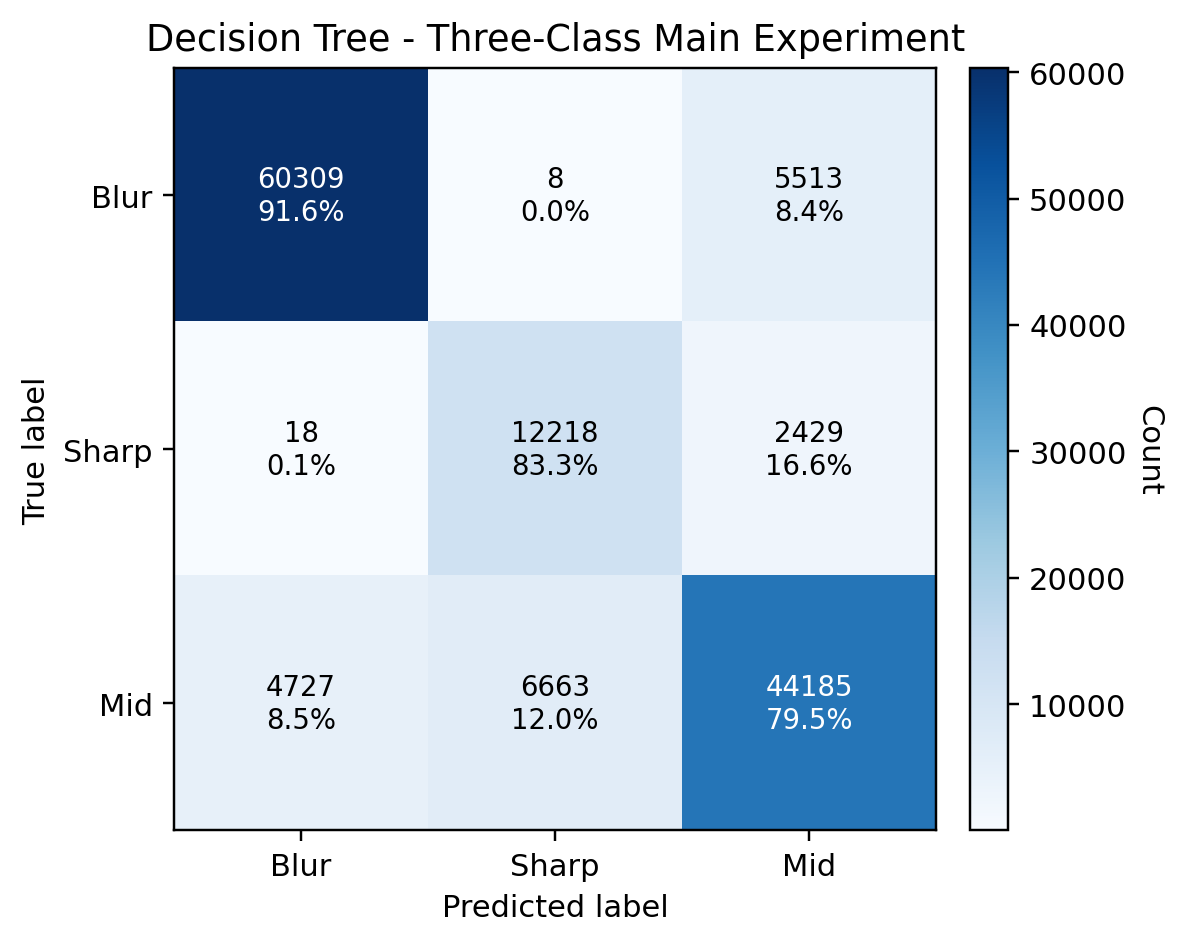
\includegraphics[width=\linewidth]{images/cm_main_3c_decision_tree.png}
        \caption{Decision Tree}
    \end{subfigure}
    \hfill
    \begin{subfigure}{0.47\textwidth}
        \centering
        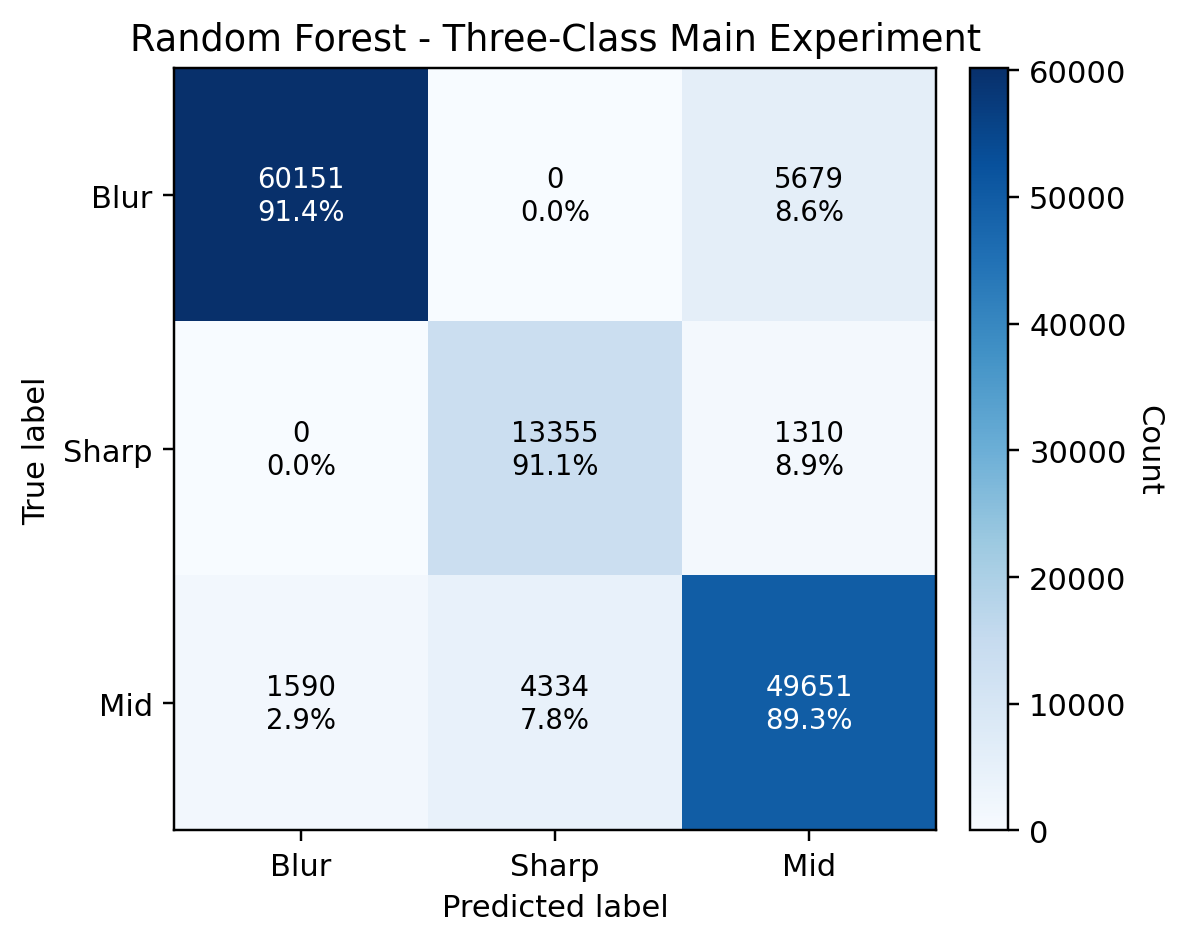
\includegraphics[width=\linewidth]{images/cm_main_3c_random_forest.png}
        \caption{Random Forest}
    \end{subfigure}

    \vspace{0.6em}

    \begin{subfigure}{0.47\textwidth}
        \centering
        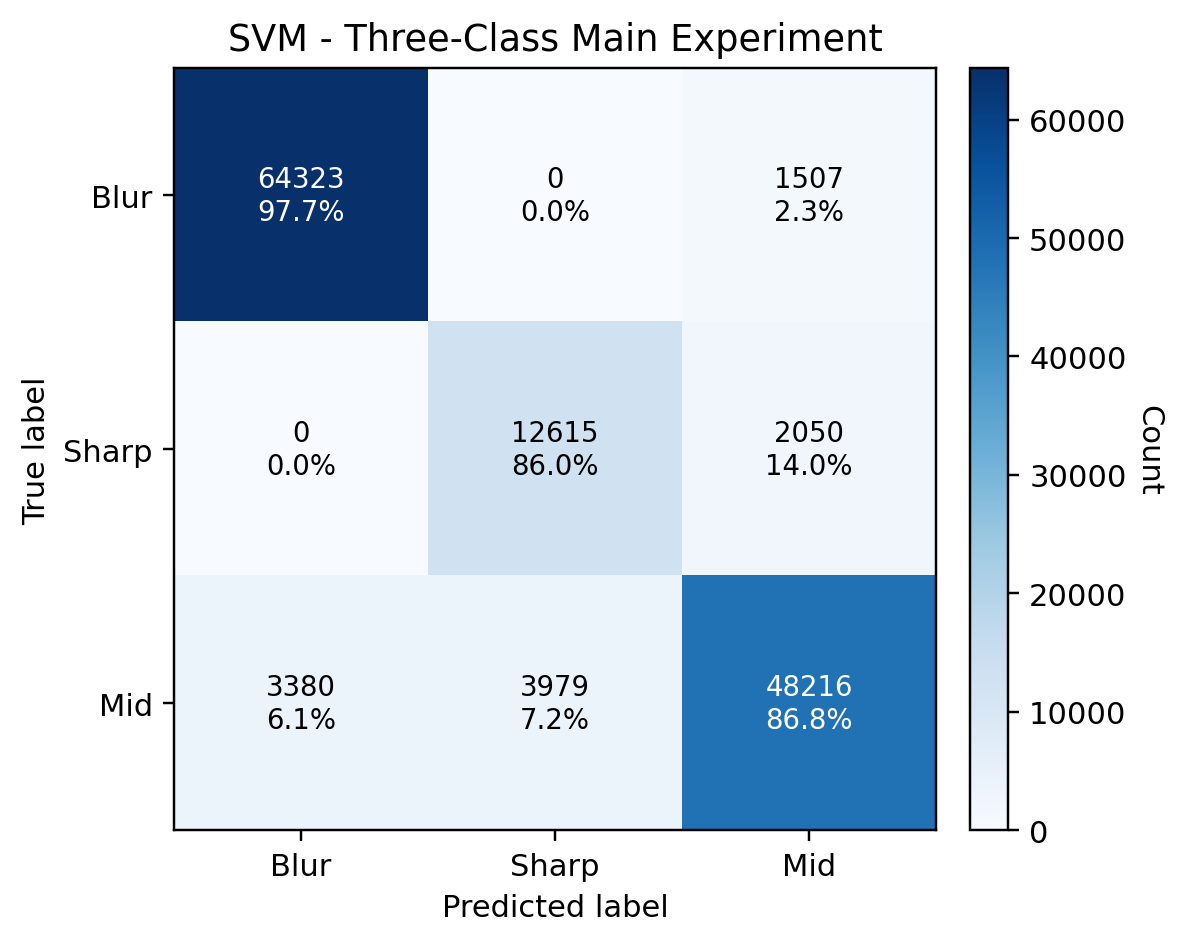
\includegraphics[width=\linewidth]{images/cm_main_3c_svm.png}
        \caption{SVM}
    \end{subfigure}
    \hfill
    \begin{subfigure}{0.47\textwidth}
        \centering
        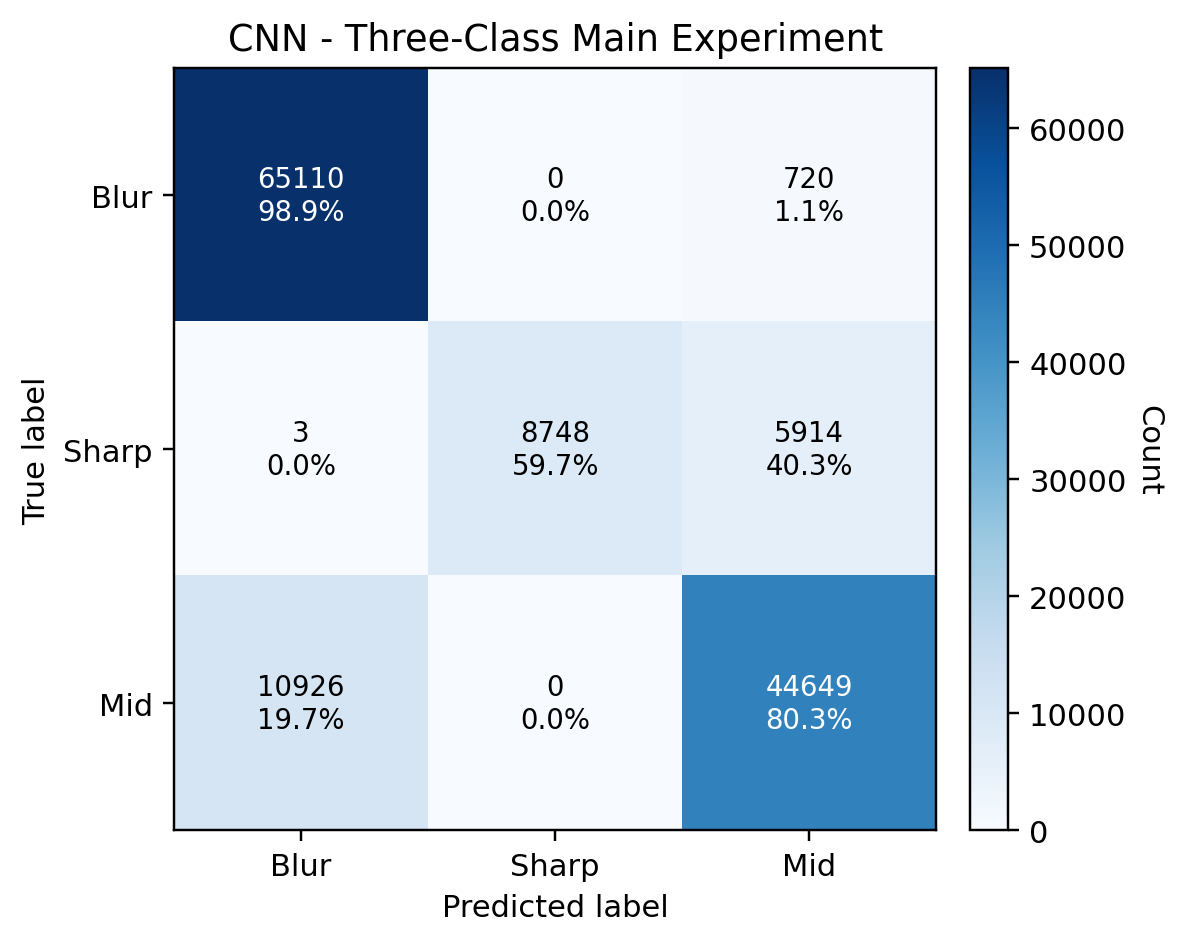
\includegraphics[width=\linewidth]{images/cm_main_3c_cnn.png}
        \caption{CNN}
    \end{subfigure}
    \caption{Confusion matrices of the four models under $100\%$ training samples in the main three-class experiment}
    \label{fig:cm-main-3c}
\end{figure}

\par Compared with the binary task, the learning difficulty of the three-class
task is clearly higher. The best sharp-class F1-score in the three-class task
is $0.83$ from random forest, while the CNN can reach $0.84$ in the binary
task. More importantly, the macro F1 of all models in the three-class setting
is lower overall than in the binary setting. At the same time, the recall of
the CNN on the sharp class in the three-class task is only $0.60$, which is
significantly lower than its $0.73$ in the binary task. This indicates that
after the intermediate-state class is separated as an independent category,
the model needs not only to distinguish the sharp class from the non-sharp
class, but also to deal with transition samples with more ambiguous
boundaries, and the task complexity increases clearly.

\par Figure~\ref{fig:cm-main-3c} shows the confusion matrices of the four models
in the main three-class experiment under $100\%$ training samples. Compared
with the binary task, the off-diagonal items are clearly more numerous in the
three-class task, which indicates that after introducing the intermediate-state
class, the model needs not only to distinguish sharp and non-sharp regions, but
also to further handle transition samples with more ambiguous boundaries. From
the overall observation, the four models all recognize the blur class
relatively stably, while the confusion between the sharp class and the
intermediate-state class becomes the main source of error.

\par A further comparison of the confusion matrices shows that the key
difficulty in the three-class task is not the direct confusion between the
sharp class and the blur class, but mainly the confusion between the sharp
class and the intermediate-state class. Taking real sharp-class samples as an
example, random forest, SVM, and decision tree almost never directly classify
them as blur, and the CNN only makes $3$ such errors. The dominant error is
instead that real sharp-class samples are predicted as intermediate-state,
where the numbers are $2429$ for decision tree, $2050$ for SVM, $1310$ for
random forest, and as high as $5914$ for CNN. This indicates that under the
three-class setting, the CNN forms an obviously conservative decision
boundary, that is, it predicts the sharp class only when the confidence is
very high, while a large number of boundary regions are contracted into the
intermediate-state class, causing sharp-class recall to decrease clearly. On
the other hand, although random forest performs best on sharp-class recall and
F1-score, it misclassifies $4334$ real intermediate-state patches as sharp.
This means that its prediction strategy is more aggressive. The higher recall
is therefore not obtained without cost, but is exchanged for more
``intermediate-state $\rightarrow$ sharp'' errors. The SVM shows a more
balanced error structure between the two: its detection of the sharp class is
relatively stable, and its macro F1 is also more stable overall, which gives
it strong comprehensive stability in the three-class task.

\par In the three-class results, the SVM shows the strongest overall stability.
Its macro F1 remains around $0.89$ in all five experiments, and its sharp-
class F1-score also stays at $0.81$. This indicates that Nystr\"{o}m-SVM has
strong generalization ability under the current hand-crafted feature and PCA
representation, and can learn the decision boundary among the three classes
relatively sufficiently even on smaller training sets. Random forest is more
prominent on sharp-class metrics: its sharp-class F1-score rises from $0.82$
to $0.83$, and its recall increases from $0.80$ to $0.91$, which makes it the
most aggressive traditional model for sharp-class detection in the three-class
task. However, as the sample size increases, its precision falls from $0.85$
to $0.75$, and therefore macro F1 does not increase correspondingly. Although
the decision tree also improves steadily as sample size increases, its final
sharp-class F1-score is only $0.73$, which is still clearly behind random
forest and SVM. From the perspective of time, the advantage of the SVM in the
three-class task is even more meaningful in practice: under $100\%$ samples,
its training time is $92.03$s, which is clearly lower than random forest's
$119.84$s and far lower than CNN's $686.11$s, while still keeping the most
stable macro F1. Therefore, the SVM in the three-class task is not only a
stable model in performance, but also a relatively efficient model in terms of
time.

\par The performance of the CNN in the three-class task is in clear contrast
with its performance in the binary task. Although its precision remains almost
$1.00$ in all five experiments, its sharp-class recall gradually drops from
$0.70$ to $0.60$, and its sharp-class F1-score also declines from $0.82$ to
$0.75$. This indicates that the model becomes more and more inclined to
predict the sharp class only at very high confidence. In other words, the CNN
learns a very conservative decision boundary in the three-class task: it can
avoid misclassifying blur or intermediate-state patches as sharp, but at the
cost of missing a large number of real sharp patches. Even at $100\%$ samples,
its sharp-class F1-score is still clearly lower than random forest's $0.83$
and SVM's $0.81$. Considering that its training time increases from $143.54$s
to $686.11$s, this indicates that under the current network structure and
training strategy, the deep model has not yet fully shown its advantage in the
three-class setting.

\par Overall, in the three-class task, if stability of macro F1 and class
balance is the first priority, the SVM is the most suitable main model. If
sharp-class recall and F1-score are emphasized more, random forest has better
sharp-class detection ability. Although the CNN performs best in the binary
task, its recognition of the sharp class is still too conservative in the
three-class task. If its performance is to be further improved in the future,
stronger data augmentation, class reweighting, or specialized threshold
calibration may be needed.

\section{Sample-Size Analysis}
\par To analyze the role of training data scale more systematically, this
section treats the scan result from $20\%$ to $100\%$ samples as an
independent dimension for discussion. Compared with only comparing the final
results under a single training ratio, sample-size analysis can better reveal
the speed of learning saturation, the sensitivity of models to data volume,
and whether the performance improvement is worth the additional computational
cost.

\subsection{Class Distribution and Scaling}
\par From the training data distribution, the binary task keeps a stable
imbalanced structure across all five training ratios. Taking the $100\%$
training set as an example, the number of non-sharp and sharp samples is
$578212$ and $59941$, respectively, and the sharp class accounts for only
about $9.39\%$. In the $20\%$ training set, the corresponding numbers are
$115735$ and $11896$, and the ratio remains basically the same. This indicates
that the change in training sample ratio mainly affects the total sample
number, but does not change the class proportion. Therefore, the performance
change can mainly be attributed to the training sample quantity itself rather
than to a change in class distribution. The three-class task shows a similar
stable distribution. Under the $100\%$ training set, the blur, sharp, and
intermediate-state classes contain $320810$, $59941$, and $257402$ samples,
respectively. The sharp class still accounts for only about $9.39\%$, while
the blur class accounts for about $50.27\%$ and the intermediate-state class
for about $40.34\%$. This means that the three-class task not only has the
minority-class detection problem, but also needs to establish a stable boundary
between two large non-sharp-related classes, and is therefore more difficult
than the binary setting. The evaluation curves of the four models under
different training ratios in the binary task are shown in
Fig.~\ref{fig:sample-size-2c-eva}.

\begin{figure}[htbp]
    \centering

    \begin{subfigure}{0.47\textwidth}
        \centering
        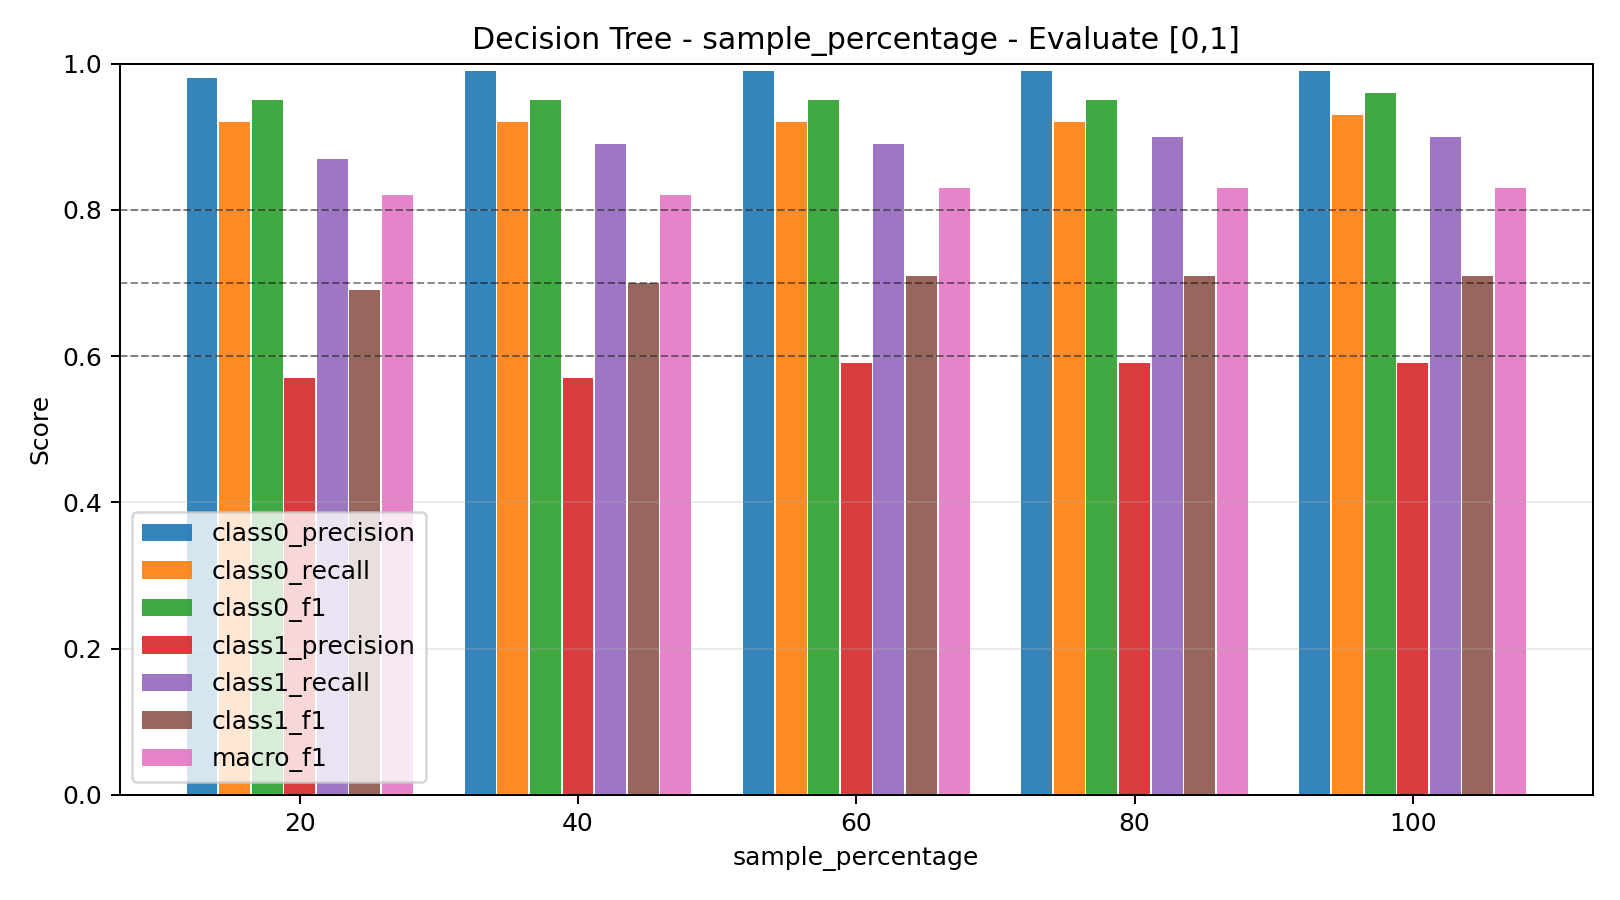
\includegraphics[width=\linewidth]{images/DT_EVA_2C}
        \caption{Decision Tree}
        \label{fig:dt-eva-2c}
    \end{subfigure}
    \hfill
    \begin{subfigure}{0.47\textwidth}
        \centering
        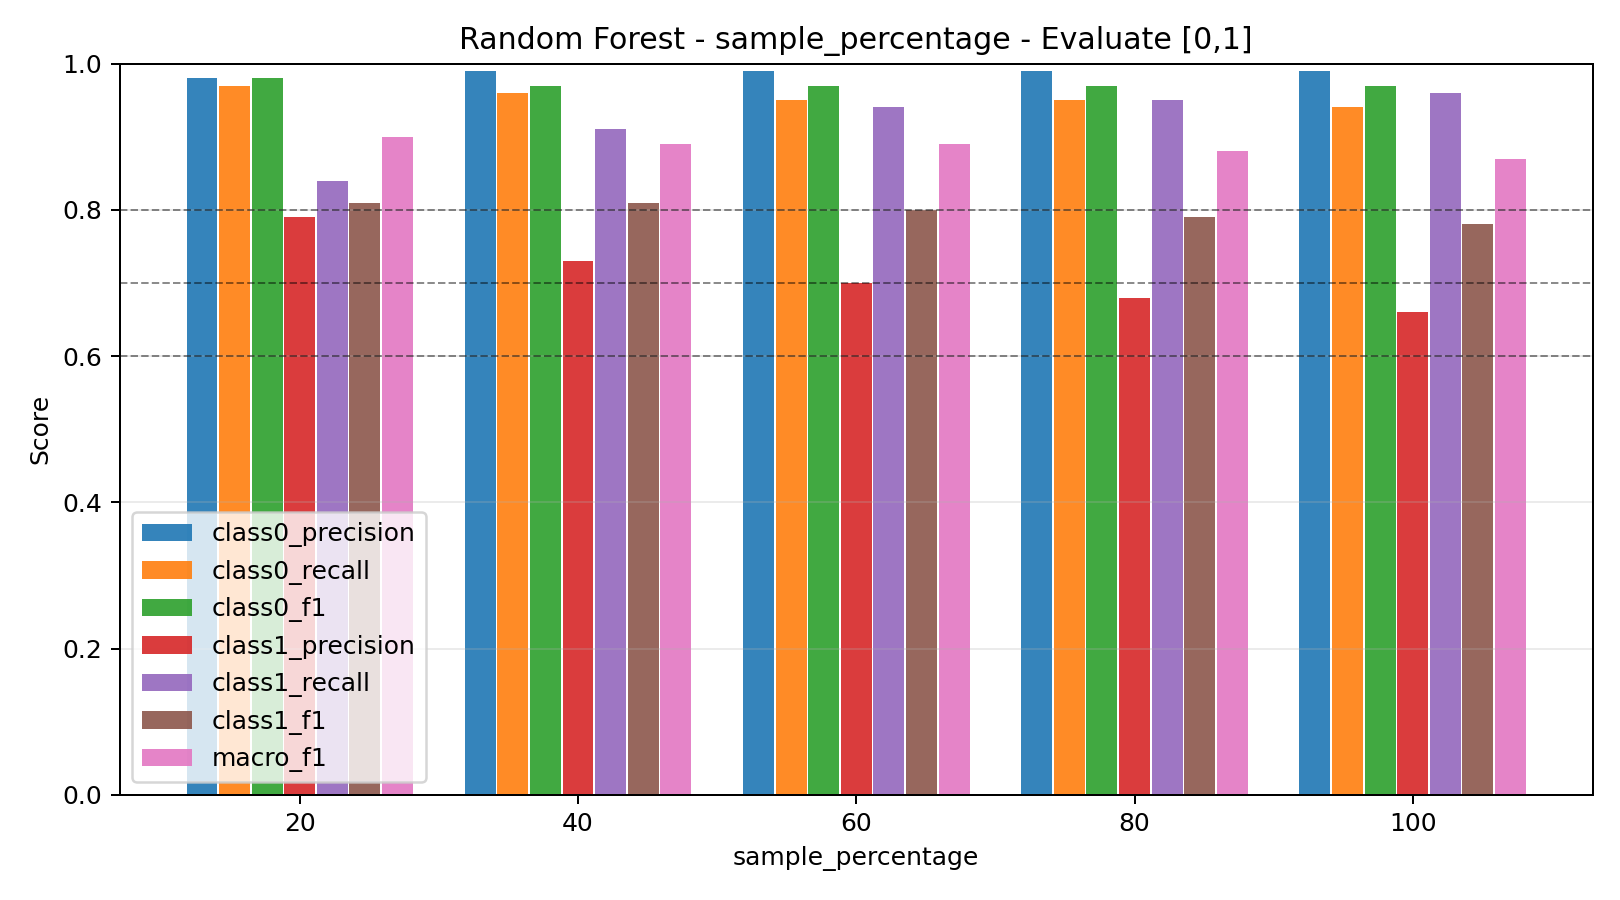
\includegraphics[width=\linewidth]{images/RF_EVA_2C}
        \caption{Random Forest}
        \label{fig:rf-eva-2c}
    \end{subfigure}

    \vspace{0.6em}

    \begin{subfigure}{0.47\textwidth}
        \centering
        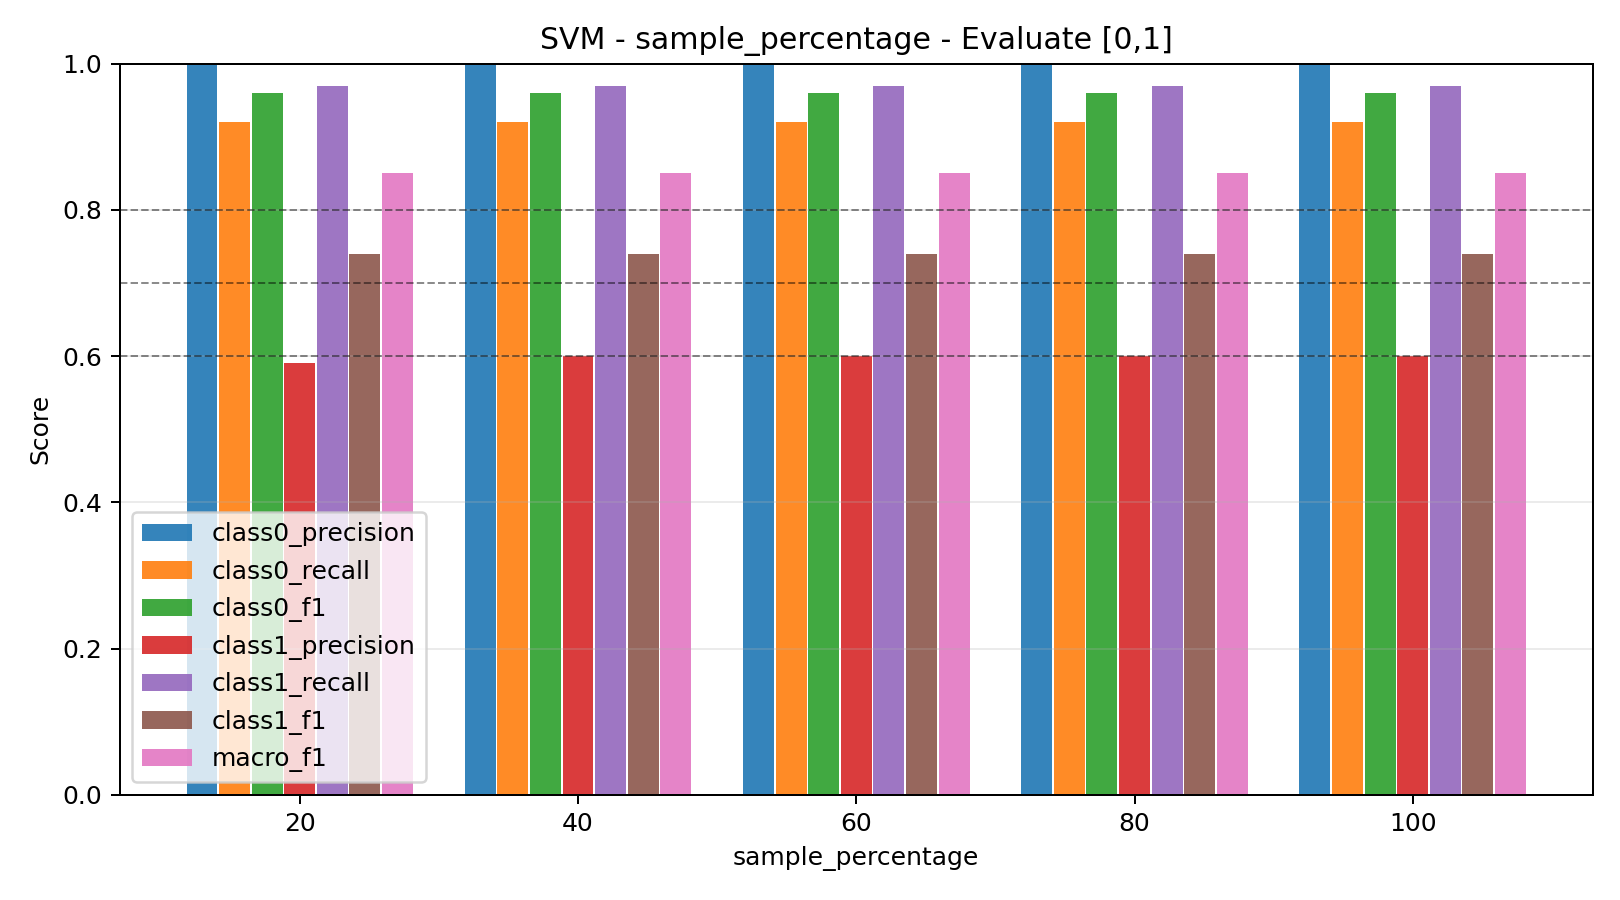
\includegraphics[width=\linewidth]{images/SVM_EVA_2C}
        \caption{SVM}
        \label{fig:svm-eva-2c}
    \end{subfigure}
    \hfill
    \begin{subfigure}{0.47\textwidth}
        \centering
        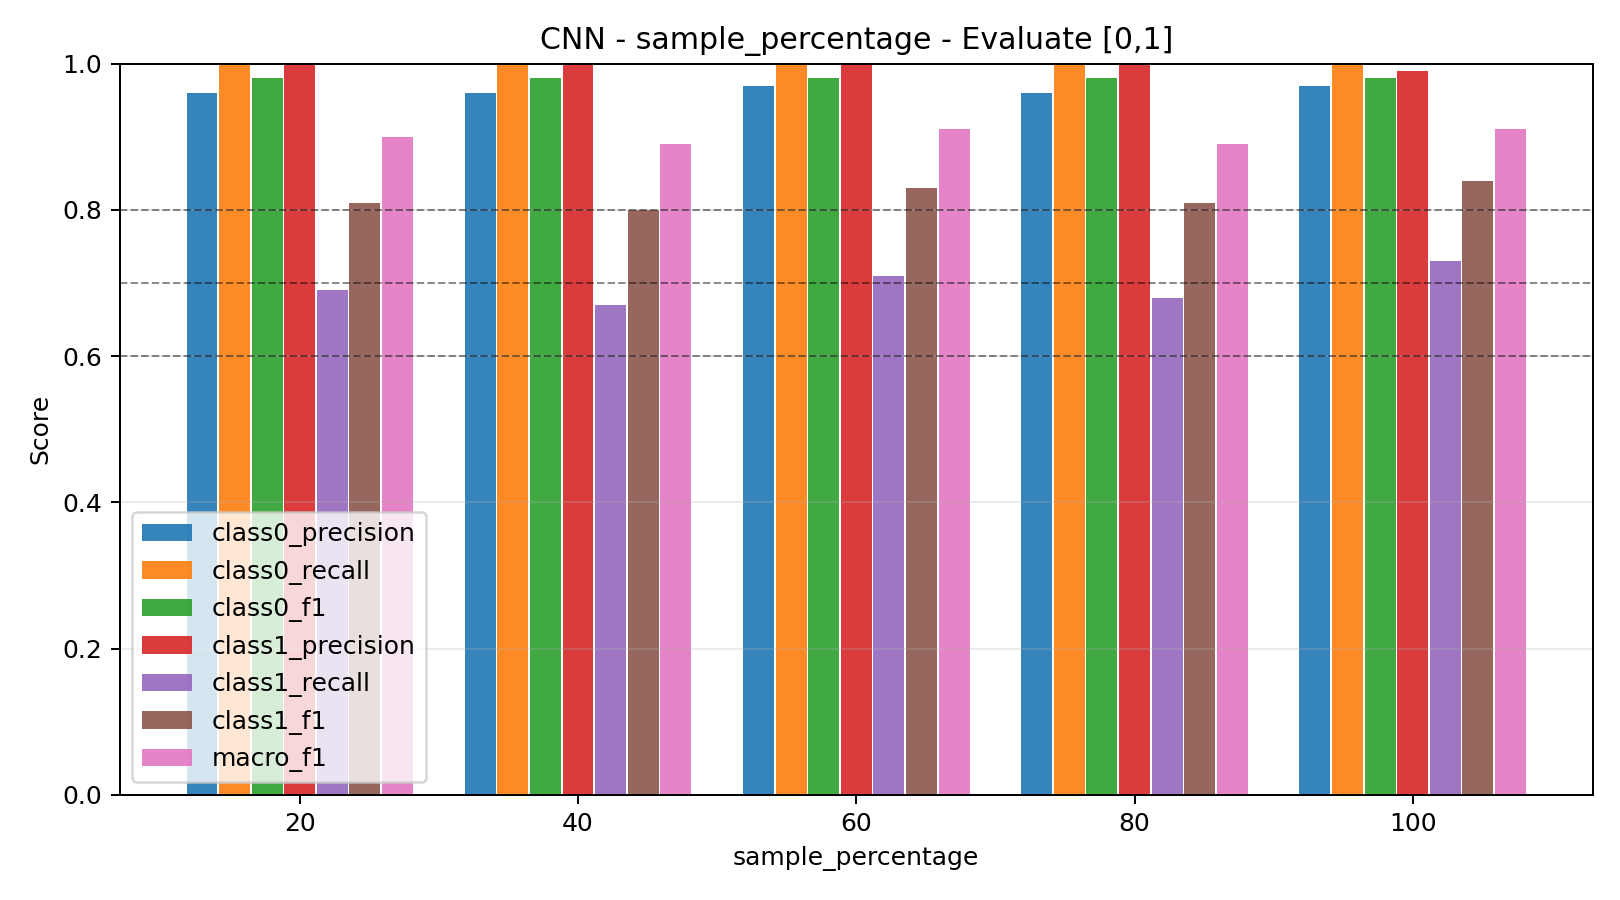
\includegraphics[width=\linewidth]{images/CNN_EVA_2C}
        \caption{CNN}
        \label{fig:cnn-eva-2c}
    \end{subfigure}

    \caption{Changes of evaluation metrics of the four models under different training ratios in the binary task}
    \label{fig:sample-size-2c-eva}
\end{figure}

\par In the binary task, whether classical machine learning models or deep
learning models are considered, as the training sample ratio increases from
$20\%$ to $100\%$, the changes in all metrics are generally not dramatic, and
most curves show only slight fluctuation or slow improvement. This indicates
that under the current feature representation, network structure, and data
distribution, increasing sample size can indeed bring some benefit, but it is
not the dominant factor determining model performance. By comparison, the
discrimination mechanism of the model itself, the complexity of the class
boundary, and the precision-recall trade-off affect the final result more
directly. At the same time, the training time increases almost monotonically
with the sample ratio. Therefore, when the gain is limited, whether it is
worth continuing to enlarge the sample size must be judged from both the
performance increment and the time cost.

\subsection{Binary Setting}
\par Table~\ref{tab:sample-binary-summary} summarizes the sharp-class F1-score
of each model under different training ratios in the binary task, together with
the best sharp-class F1-score at each ratio, so as to observe the main trend of
different models as data scale changes.

\begin{table}[htbp]
    \centering
    \caption{Changes of sharp-class F1-score under different training ratios in the binary task}
    \label{tab:sample-binary-summary}
    \begin{tabular}{cccccc}
        \toprule
        Sample (\%) & Decision Tree & Random Forest & SVM & CNN & Best Focus F1
        \\
        \midrule
        20  & 0.69 & 0.81 & 0.74 & 0.81 & 0.81 (RF/CNN) \\
        40  & 0.70 & 0.81 & 0.74 & 0.80 & 0.81 (RF) \\
        60  & 0.71 & 0.80 & 0.74 & 0.83 & 0.83 (CNN) \\
        80  & 0.71 & 0.79 & 0.74 & 0.81 & 0.81 (CNN) \\
        100 & 0.71 & 0.78 & 0.74 & 0.84 & 0.84 (CNN) \\
        \bottomrule
    \end{tabular}
\end{table}

\par First, from the sharp-class F1-score, the improvement of the decision tree
across the five experiments is the most limited, increasing only slowly from
$0.69$ to $0.71$, which indicates that this model has weak ability to benefit
from additional data and enters a performance saturation stage relatively
early. Random forest already reaches $0.81$ at $20\%$ samples, and then
instead slowly declines to $0.78$. This does not mean that the model
degenerates, but rather that as more data are added, it becomes more inclined
to improve sharp-class recall, which causes precision to keep decreasing and
thus lowers F1-score. The SVM is almost unaffected by training scale, with its
sharp-class F1-score remaining at $0.74$ throughout, showing very strong
stability. In contrast, the CNN fluctuates the most, but its overall increase
is also the largest: its sharp-class F1-score already rises to $0.83$ at
$60\%$ samples, and further reaches $0.84$ at $100\%$ samples. This indicates
that the deep model can indeed continue to improve its representation ability
with a larger training set. However, if time is considered at the same time,
the cost of this improvement is high: its training time increases from
$143.14$s to $684.51$s, while the sharp-class F1-score only rises from $0.81$
to $0.84$, which indicates that the marginal gain brought by increasing sample
size is relatively limited.

\par Second, from the ownership of the best sharp-class F1-score, there is no
single dominant model in the binary task under smaller data scale. At $20\%$
samples, random forest and CNN both achieve a sharp-class F1-score of $0.81$.
At $40\%$ samples, random forest is slightly better. When the training ratio
increases to $60\%$ and above, however, the CNN begins to dominate stably and
reaches the highest value of the whole group, $0.84$, at $100\%$ samples. This
indicates that even under smaller data scale, the deep model can already rely
on high precision to achieve an F1-score comparable to traditional methods. As
data scale continues to increase, its precision advantage can gradually be
converted into stronger overall F1 performance. However, if the sharp-class
recall is further examined, it can be seen that even at $100\%$ samples, the
recall is still only $0.73$, which is clearly lower than the SVM's $0.97$ and
random forest's $0.96$. Therefore, for this task, even when F1-score is used
as the main metric, recall still needs to be examined at the same time, in
order to avoid a model obtaining a seemingly high F1 simply through an overly
conservative prediction strategy.

\par Finally, from the growth trend of computational cost, the training time of
all four models in the binary task increases significantly with sample size,
but the growth slope differs greatly. Decision tree increases from $17.98$s to
$103.48$s, random forest from $19.46$s to $120.80$s, and CNN from $143.14$s
to $684.51$s, all close to a factor of $5$. By contrast, the SVM increases
only from $3.64$s to $17.68$s and has the lowest absolute cost. This shows
that in the binary setting, the SVM is the most scalable traditional model,
while the CNN, although best on accuracy and F1, is also the most expensive.
Therefore, if more ablation studies or larger-scale experiments are needed in
the future, the SVM is more suitable as a high-recall, low-cost baseline.

\subsection{Three-Class Setting}
\par The change of the sharp-class F1-score under different training ratios in
the three-class task is shown in
Table~\ref{tab:sample-triclass-summary}.

\begin{table}[htbp]
    \centering
    \caption{Changes of sharp-class F1-score under different training ratios in the three-class task}
    \label{tab:sample-triclass-summary}
    \begin{tabular}{cccccc}
        \toprule
        Sample (\%) & Decision Tree & Random Forest & SVM & CNN & Best Focus F1
        \\
        \midrule
        20  & 0.70 & 0.82 & 0.81 & 0.82 & 0.82 (RF/CNN) \\
        40  & 0.71 & 0.83 & 0.81 & 0.77 & 0.83 (RF) \\
        60  & 0.73 & 0.83 & 0.81 & 0.77 & 0.83 (RF) \\
        80  & 0.73 & 0.83 & 0.81 & 0.76 & 0.83 (RF) \\
        100 & 0.73 & 0.83 & 0.81 & 0.75 & 0.83 (RF) \\
        \bottomrule
    \end{tabular}
\end{table}

\par The evaluation curves of the four models under different training ratios
in the three-class task are shown in Fig.~\ref{fig:sample-size-3c-eva}.

\begin{figure}[htbp]
    \centering

    \begin{subfigure}{0.47\textwidth}
        \centering
        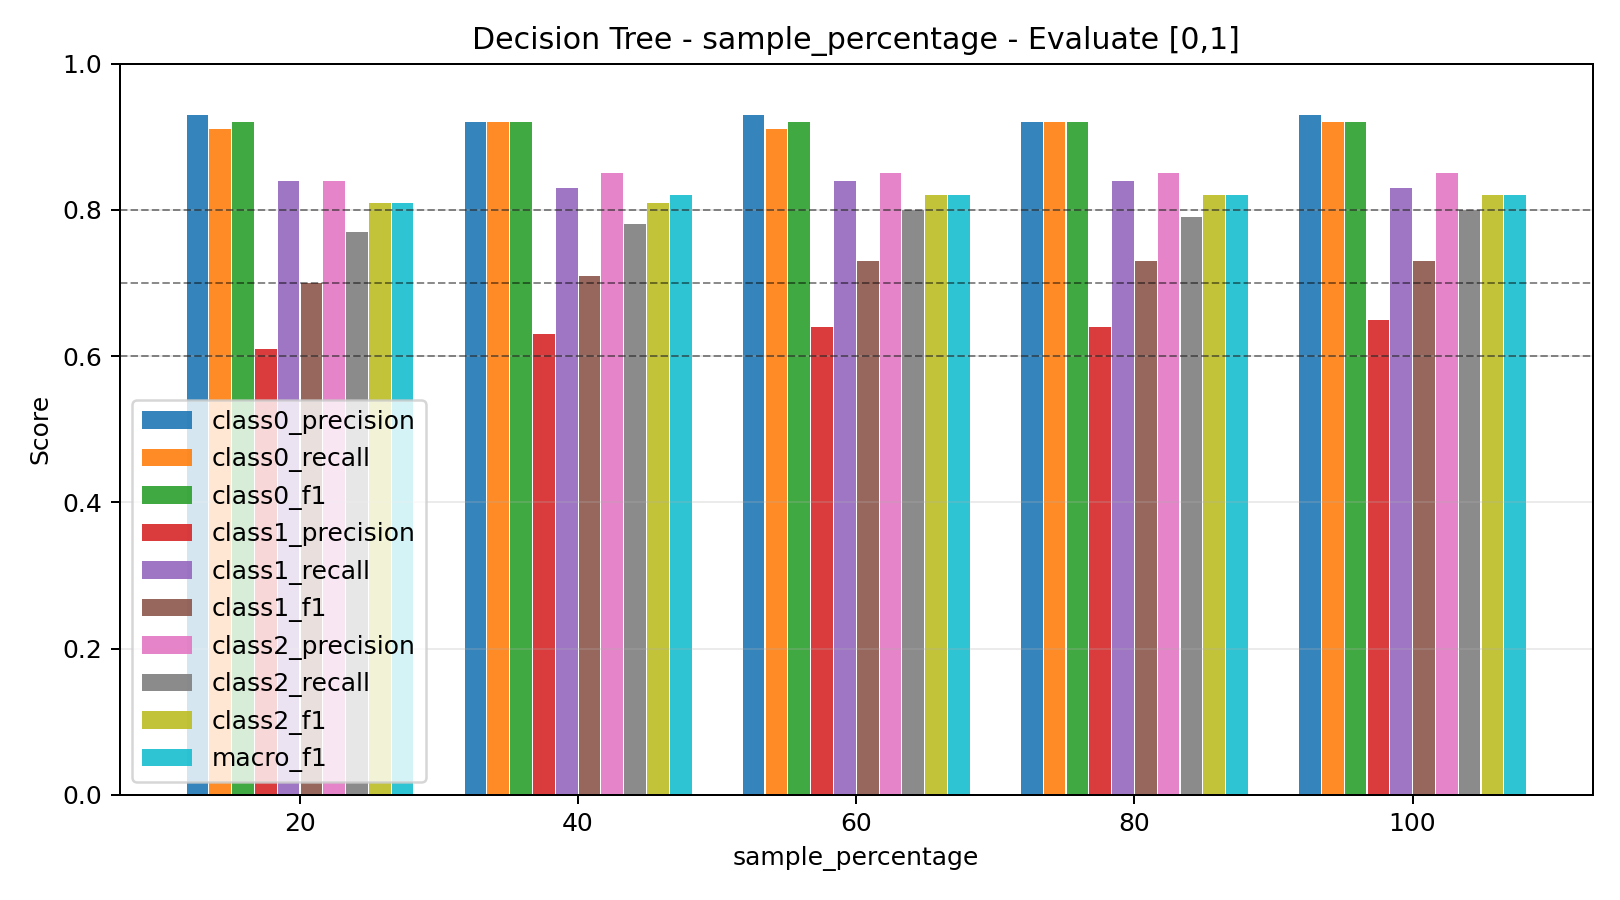
\includegraphics[width=\linewidth]{images/DT_EVA_3C}
        \caption{Decision Tree}
        \label{fig:dt-eva-3c}
    \end{subfigure}
    \hfill
    \begin{subfigure}{0.47\textwidth}
        \centering
        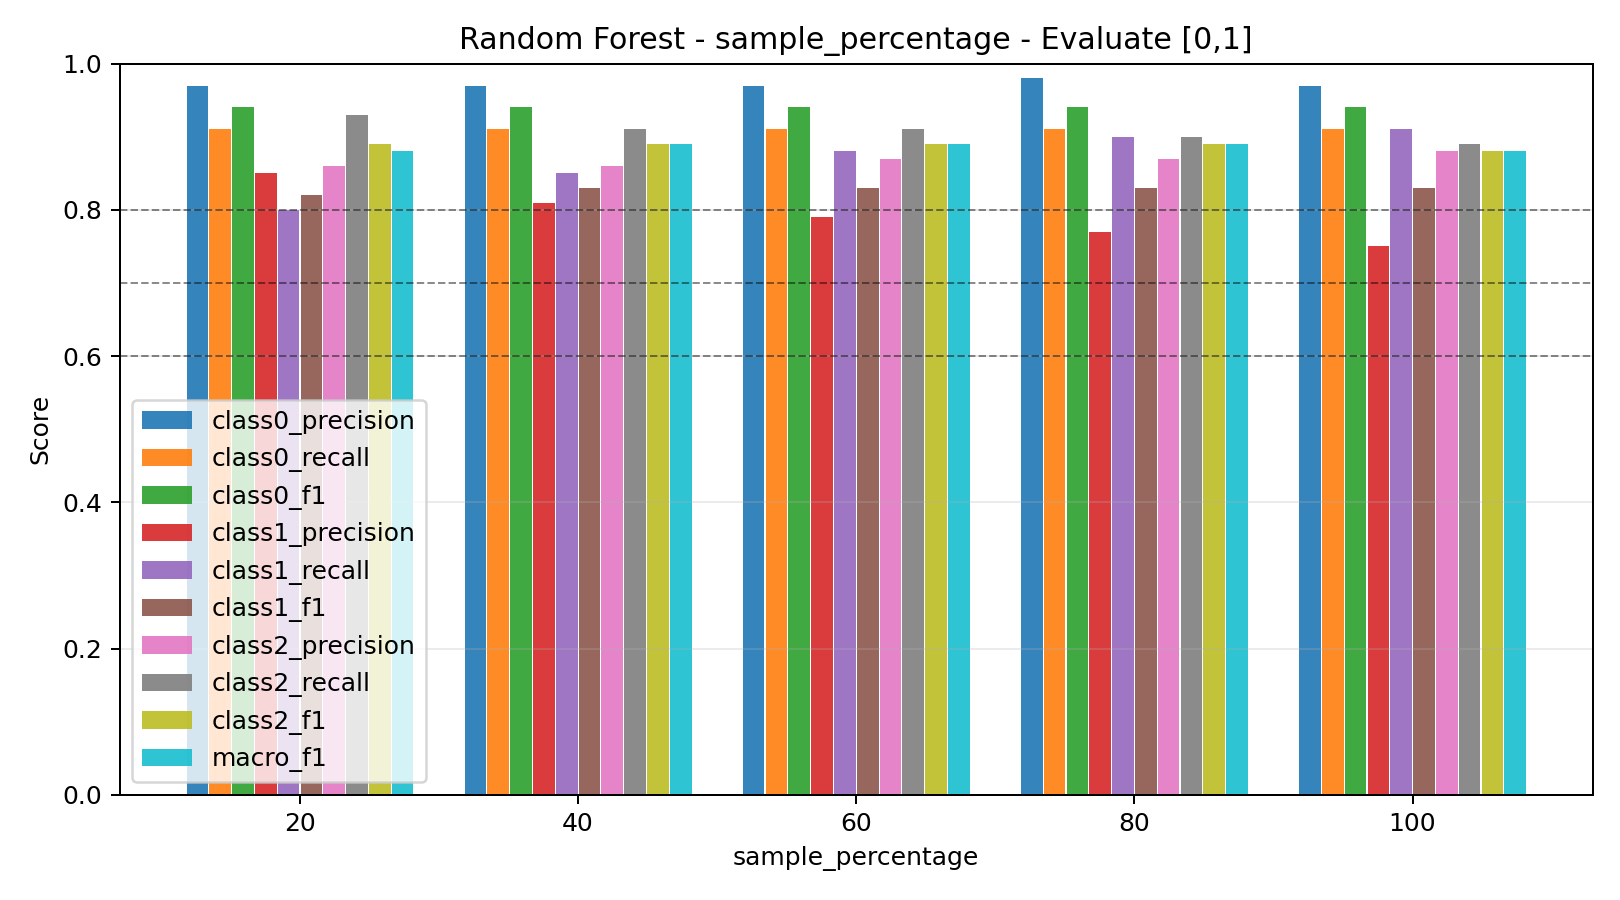
\includegraphics[width=\linewidth]{images/RF_EVA_3C}
        \caption{Random Forest}
        \label{fig:rf-eva-3c}
    \end{subfigure}

    \vspace{0.6em}

    \begin{subfigure}{0.47\textwidth}
        \centering
        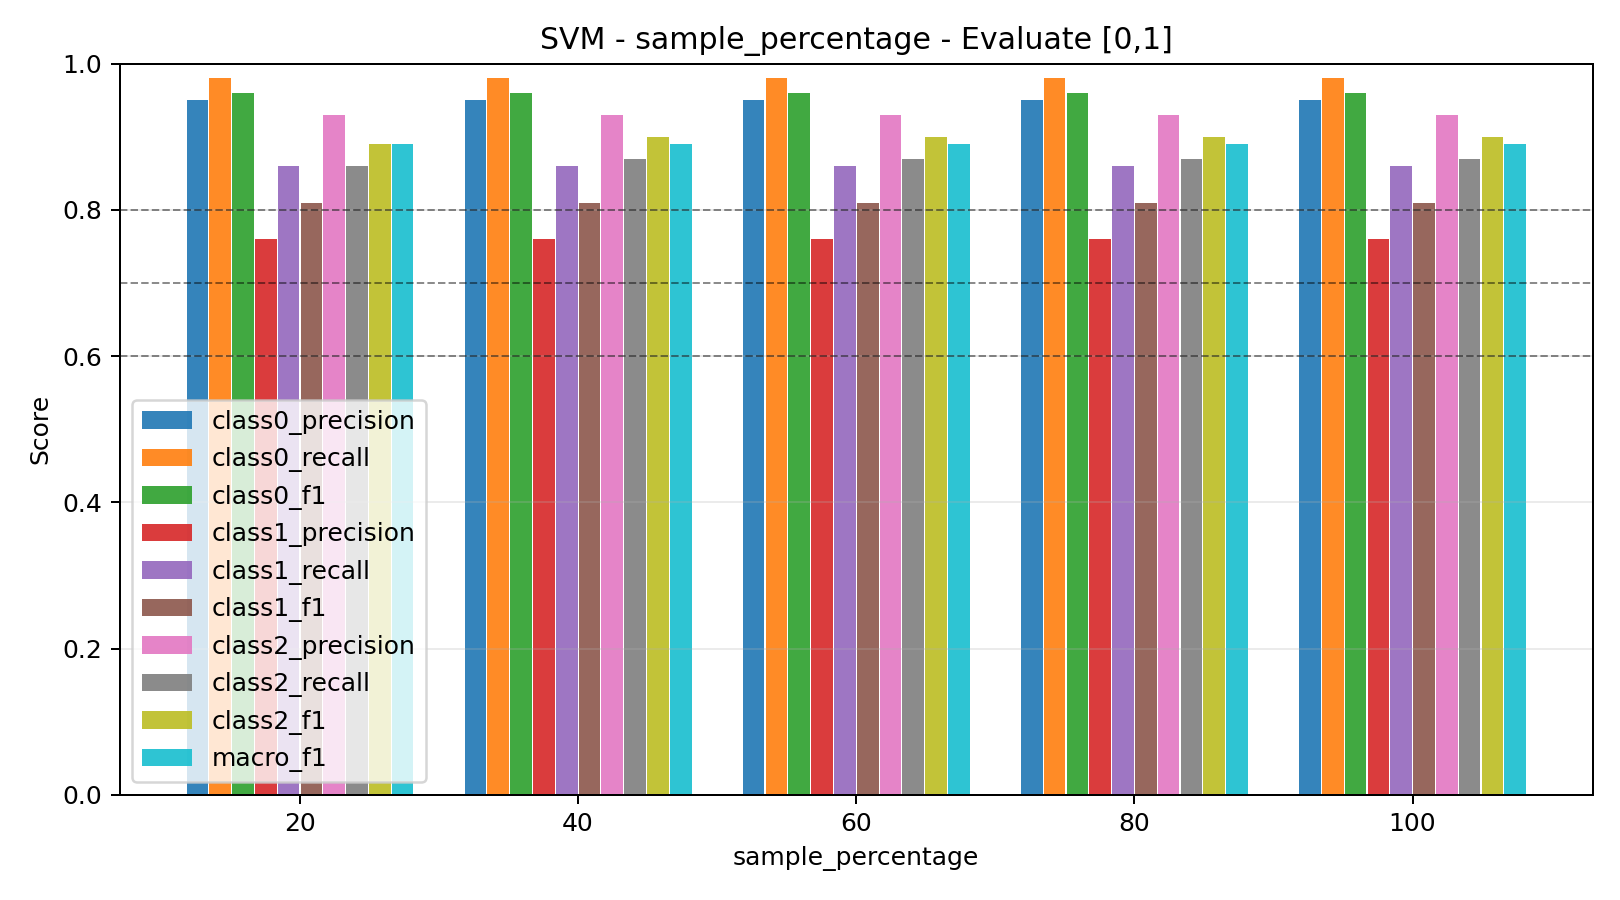
\includegraphics[width=\linewidth]{images/SVM_EVA_3C}
        \caption{SVM}
        \label{fig:svm-eva-3c}
    \end{subfigure}
    \hfill
    \begin{subfigure}{0.47\textwidth}
        \centering
        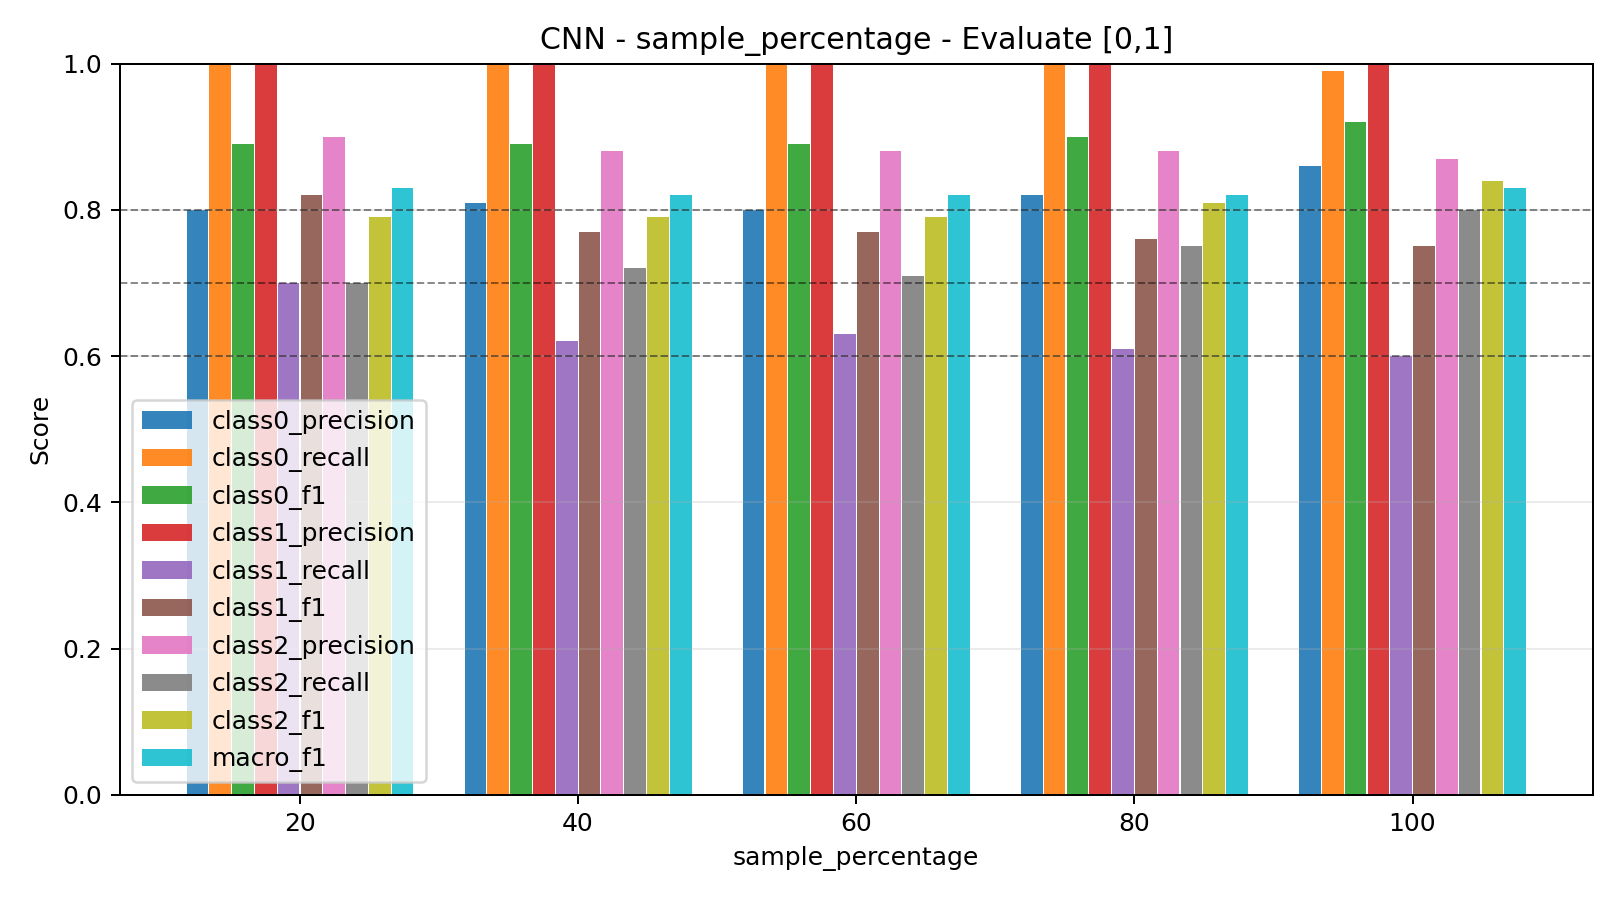
\includegraphics[width=\linewidth]{images/CNN_EVA_3C}
        \caption{CNN}
        \label{fig:cnn-eva-3c}
    \end{subfigure}

    \caption{Changes of evaluation metrics of the four models under different training ratios in the three-class task}
    \label{fig:sample-size-3c-eva}
\end{figure}

\par The overall trend in the three-class task is consistent with that in the
binary task, namely that the gain brought by increasing sample size is still
relatively limited. Most models do not show a large jump in the interval from
$20\%$ to $100\%$, but instead show slow improvement, stable plateau behavior,
or slight fluctuation. This further indicates that for the current three-class
setting, the performance bottleneck comes more from the complexity of the class
boundaries themselves, especially the similarity between the sharp class and
the intermediate-state class, rather than only from insufficient training data.
At the same time, training time continues to increase as the sample ratio
grows, which means that sample expansion in the three-class task leads to
higher time cost while performance improvement remains limited.

\par The largest difference between the three-class and binary results is that
increasing training samples does not bring a clear and consistent improvement
to all models as one might expect. The decision tree improves from $0.70$ to
$0.73$, and the increase is still limited. Random forest stays basically at
$0.83$ after $40\%$. The SVM remains stable at $0.81$ throughout all five
experiments. The CNN, in contrast, decreases continuously from $0.82$ to
$0.75$. This indicates that the main bottleneck in the three-class task is not
simply lack of data, but the greater complexity of the class boundaries
themselves, especially the strong visual similarity between the sharp class and
the intermediate-state class. For SVM and random forest, the current feature
representation is already sufficient to obtain relatively stable performance
under smaller samples, and therefore the marginal benefit of further enlarging
the training set is limited. For the CNN, more data do not automatically
translate into stronger sharp-class recognition ability, but instead make the
model more conservative at the class boundary.

\par From the ownership of sharp-class F1-score, in the three-class task,
random forest and CNN are tied for the best result at $20\%$ samples, but when
the training ratio increases to $40\%$ and above, random forest stably keeps
the highest sharp-class F1-score ($0.83$). This phenomenon has two meanings.
First, Nystr\"{o}m-SVM is well adapted to the current PCA feature space, and
therefore even when the sample scale increases, its sharp-class F1-score and
macro F1 remain mainly stable. Second, random forest uses additional samples in
a way that is more biased toward improving sharp-class detection ability, and
therefore continues to dominate on sharp-class F1-score. If the goal is to
find sharp regions as completely as possible, then the application value of
random forest in the three-class task is higher than what would be concluded
only from a single overall metric.

\par From the perspective of training cost, the growth trend of all models is
steeper in the three-class task than in the binary task. Decision tree
increases from $16.89$s to $98.61$s, random forest from $18.55$s to
$119.84$s, and CNN from $143.54$s to $686.11$s, all showing approximately
linear growth. The SVM increases from $14.52$s to $92.03$s, and this increase
is clearly larger than in the binary setting. The reason is that under the
three-class setting, the class boundaries are more complex and the optimization
difficulty of support-vector approximation mapping becomes higher. Therefore,
even with the same sample size, the training cost of the SVM increases
significantly. Even so, the SVM still keeps the most stable macro F1 and a
stable sharp-class F1-score in the three-class task, and therefore its
additional cost is still supported by the benefit in results.

\section{Supplementary Analyses}
\par In addition to the main experiments, this thesis further investigates the
role of sample rebalancing strategies in the CNN. It should be clarified that
the CNN in the main experiments of the thesis already uses loss weights
calculated according to class frequency, but does not enable weighted sampling.
Therefore, the ``weighted sampler'' discussed in this section more precisely
means enabling an additional weighted sampling strategy while keeping the loss
weights unchanged, and observing whether this can further improve the
recognition performance of the minority sharp class. Since this supplementary
experiment is only conducted on the CNN, the results of the classical models
remain unchanged.

\begin{table}[htbp]
    \centering
    \caption{Supplementary comparison before and after enabling the weighted sampler in CNN}
    \label{tab:supp-weighted-sampler}
    \begin{tabular}{llccccc}
        \toprule
        Task & Setting & Accuracy & Precision$_{\mathrm{focus}}$ &
        Recall$_{\mathrm{focus}}$ & F1$_{\mathrm{focus}}$ & Macro F1 \\
        \midrule
        Binary & No sampler (main exp.)     & 0.9709 & 0.99 & 0.73 & 0.84 & 0.91
        \\
        Binary & Weighted sampler, $t=0.5$  & 0.9666 & 1.00 & 0.69 & 0.82 & 0.90
        \\
        Binary & Weighted sampler, $t=0.3$  & 0.9697 & 1.00 & 0.72 & 0.84 & 0.91
        \\
        Three-class & No sampler (main exp.)    & 0.8709 & 1.00 & 0.60 & 0.75 &
        0.83 \\
        Three-class & Weighted sampler          & 0.8725 & 1.00 & 0.69 & 0.82 &
        0.85 \\
        \bottomrule
    \end{tabular}
\end{table}

\par From the binary results, the weighted sampler does not directly bring the
expected gain. When the default threshold $t=0.5$ is retained, the precision
of the model on the sharp class remains at $1.00$, which indicates that the
prediction strategy is still very conservative. However, recall drops from
$0.73$ to $0.69$, which causes the sharp-class F1-score to fall back from
$0.84$ to $0.82$, and macro F1 also decreases from $0.91$ to $0.90$. This
shows that under the binary setting, the loss weight in the main experiment is
already sufficient to impose a strong constraint on the minority class, and the
additional introduction of sampling reweighting does not further improve sharp-
class detection, but may instead enlarge training fluctuation. Furthermore,
after lowering the decision threshold of the sharp class in the supplementary
experiment from $0.5$ to $0.3$, the sharp-class recall rises back to $0.72$,
the sharp-class F1-score recovers to $0.84$, and macro F1 also returns to
$0.91$. This indicates that the main role of the weighted sampler in binary
classification is not to stably improve representation ability, but to change
the output score distribution. If threshold calibration is not used together
with it, the gain is not obvious.

\par The three-class result shows a different conclusion. After enabling the
weighted sampler, the sharp-class recall of the CNN clearly increases from
$0.60$ to $0.69$, the sharp-class F1-score rises from $0.75$ to $0.82$, and
macro F1 also improves from $0.83$ to $0.85$, while accuracy increases
slightly as well. This indicates that under the three-class setting, sample
reweighting does indeed alleviate the learning pressure faced by the sharp
class as a minority class, and makes the model no longer as overly
conservative as in the main experiment. Combined with the confusion matrix, it
can be seen that the weighted sampler mainly reduces the number of real
sharp-class samples that are predicted as intermediate-state, so the
improvement is not only a fluctuation of local metrics, but a direct
improvement on the most difficult class boundary.

\par Overall, the effect of the weighted sampler is clearly task-dependent. For
the binary task, additional sampling reweighting is not better than the main
experimental configuration, which indicates that ``loss weight + default
threshold'' is already sufficient. If the CNN is to be further improved later,
threshold calibration should be considered before further strengthening
sampling bias. For the three-class task, however, the weighted sampler brings a
substantial gain, which indicates that when the intermediate-state class is
introduced, the learning of the minority sharp patches by the CNN is more
easily suppressed by majority-class boundaries, and in this case strengthening
minority-class exposure through sampling rebalance is effective. Therefore, if
future work continues to focus on the three-class CNN, the weighted sampler is
recommended as a default training option rather than relying only on static
loss weights.

\section{Manual Verification of Model Outputs}
\par Before entering the overall discussion, this thesis performs additional
manual verification of the model outputs. Specifically, the thesis first
compares model performance according to quantitative metrics on the validation
set and identifies the results worth further discussion; afterwards,
representative samples are selected from the validation set, and the original
automatic labels and model outputs are compared through manual visualization.
That is, the analysis of results in this thesis follows the order of
``quantitative comparison first, manual cross-verification afterwards'', rather
than making judgments only from visual impression.

\par For the binary task, Fig.~\ref{fig:valid-2c-compare} shows the original
automatic labels and the prediction results of each model on the same
validation image. Manual verification shows that although the models differ in
local boundaries, region continuity, and a small number of fragmented patches,
the main focus regions they recover are overall consistent with the original
labels.

\begin{figure}[!htbp]
    \centering
    \begin{subfigure}[t]{0.31\textwidth}
        \centering
        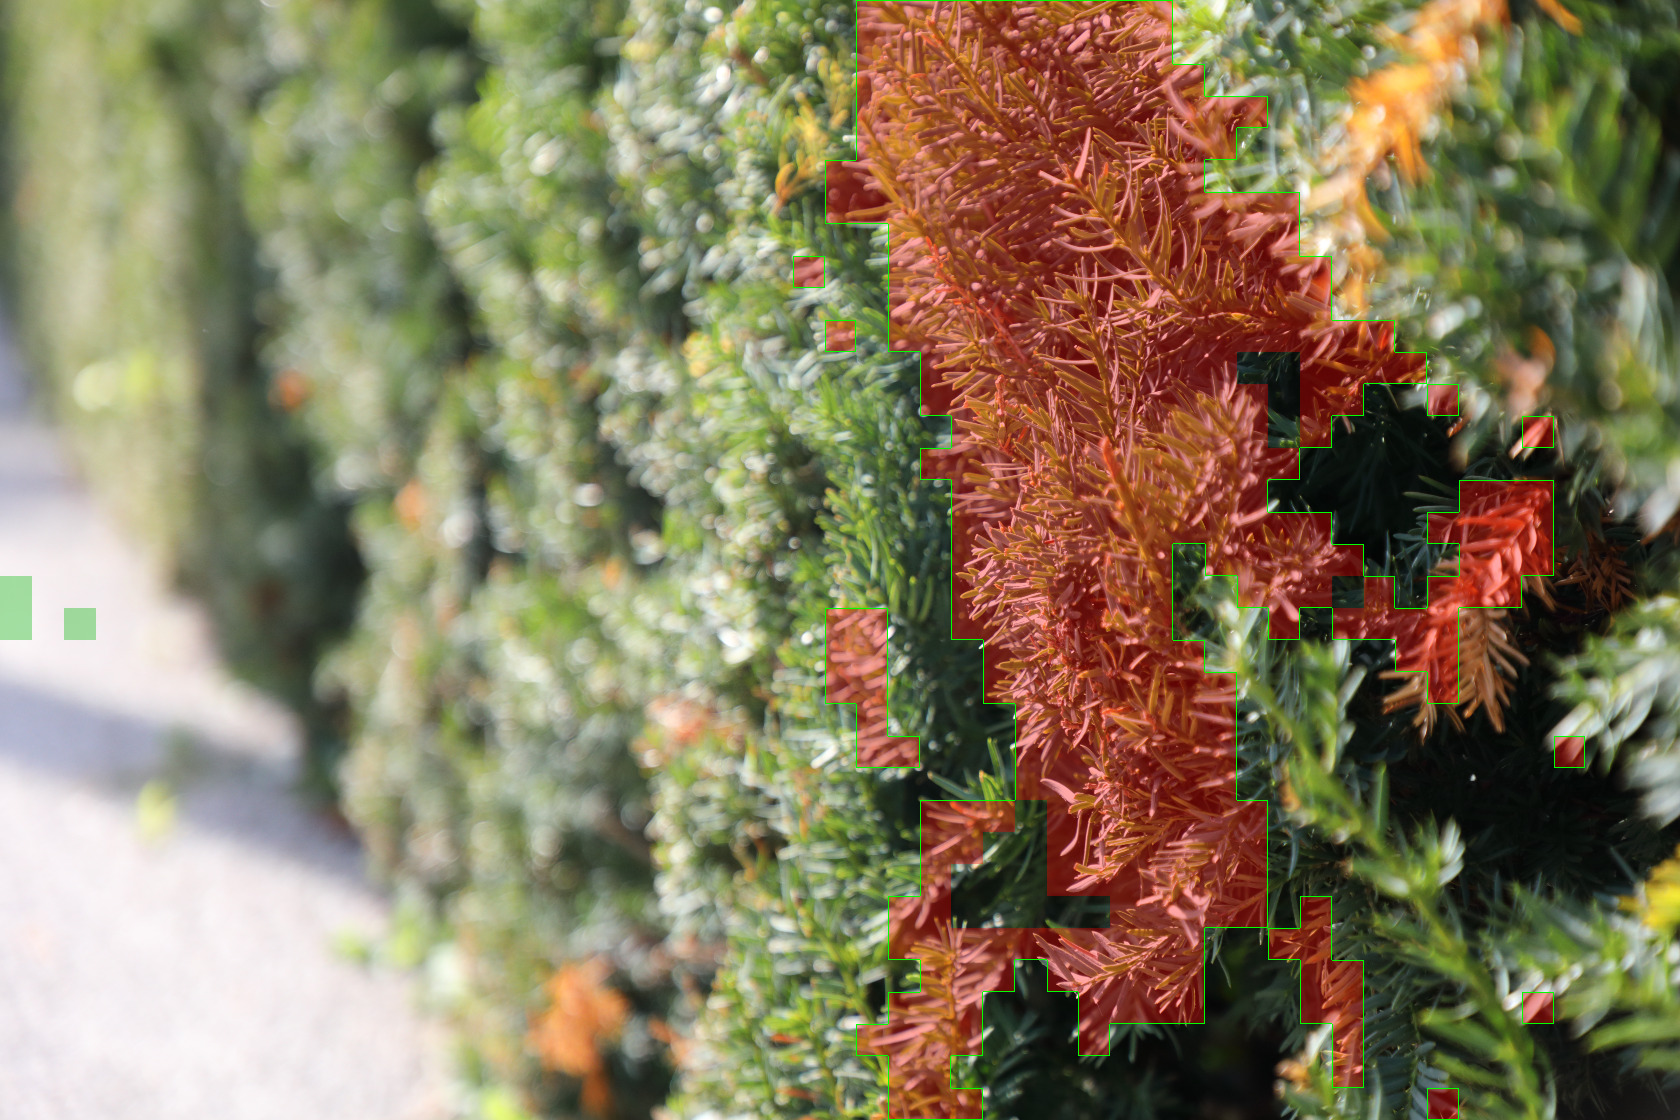
\includegraphics[width=\textwidth]{images/valid1_2C.png}
        \caption{Original auto label}
    \end{subfigure}
    \hfill
    \begin{subfigure}[t]{0.31\textwidth}
        \centering
        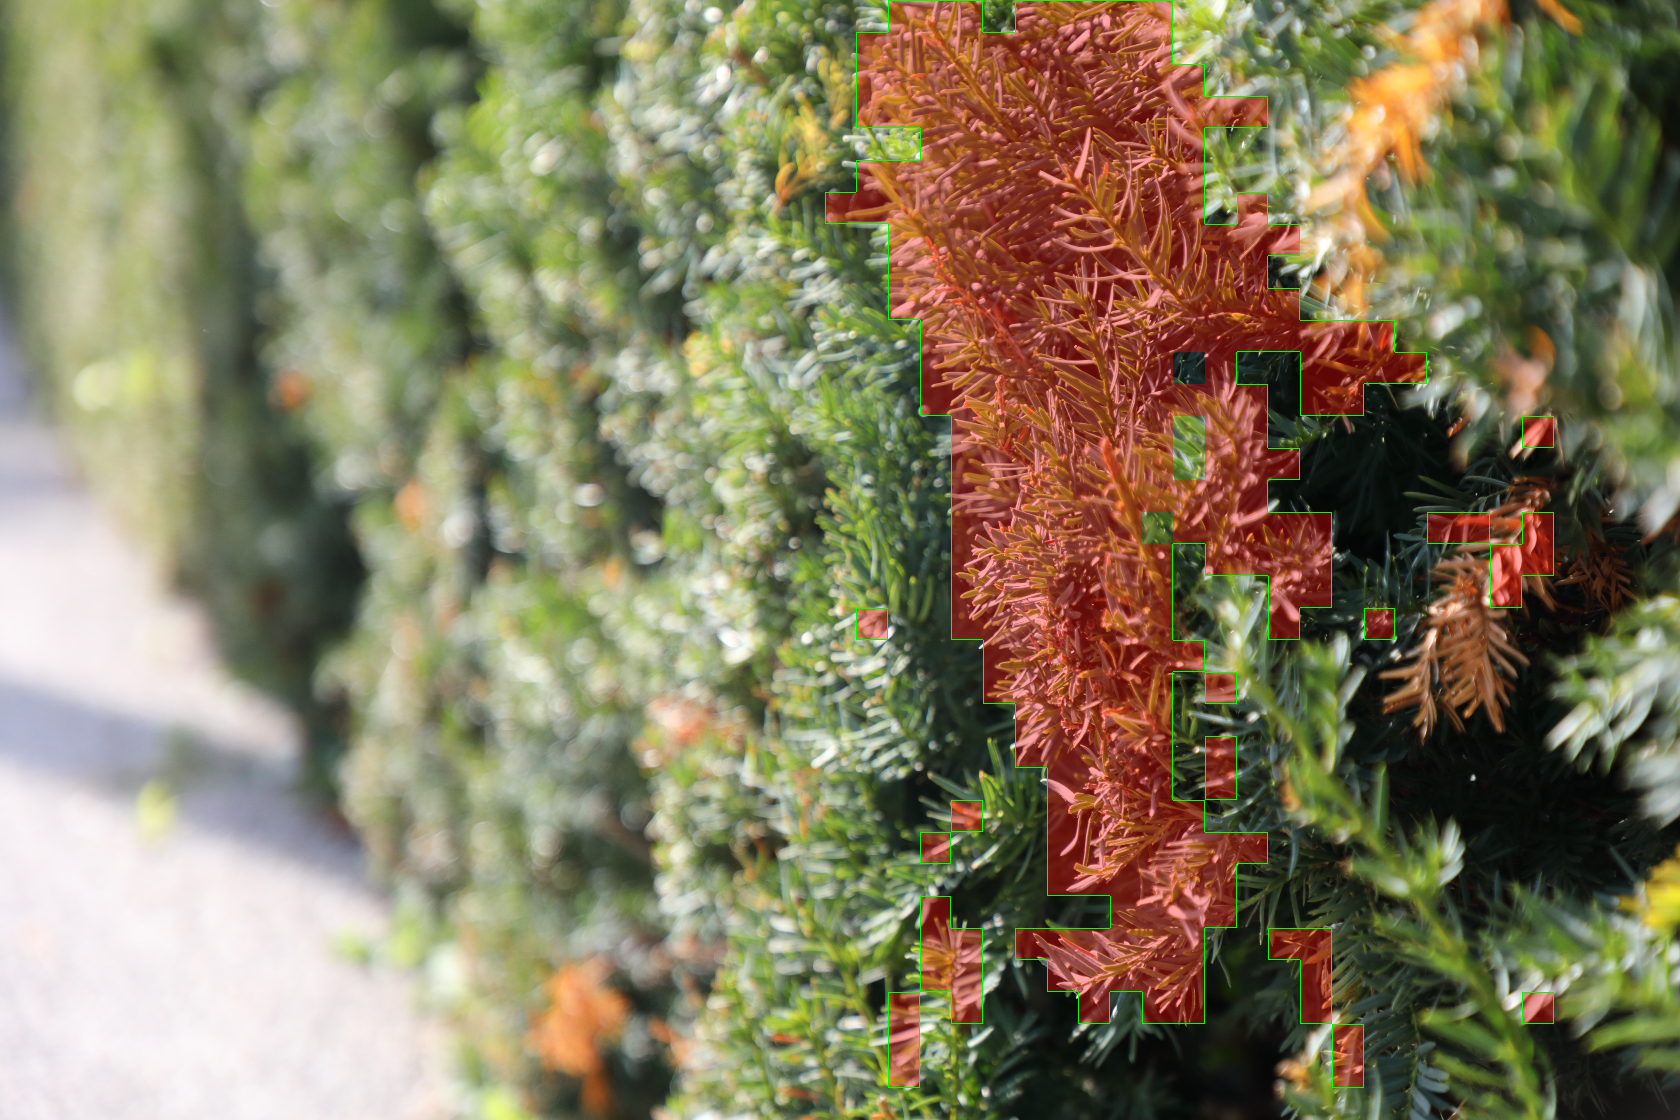
\includegraphics[width=\textwidth]{images/valid1_CNN_2C.png}
        \caption{CNN}
    \end{subfigure}
    \hfill
    \begin{subfigure}[t]{0.31\textwidth}
        \centering
        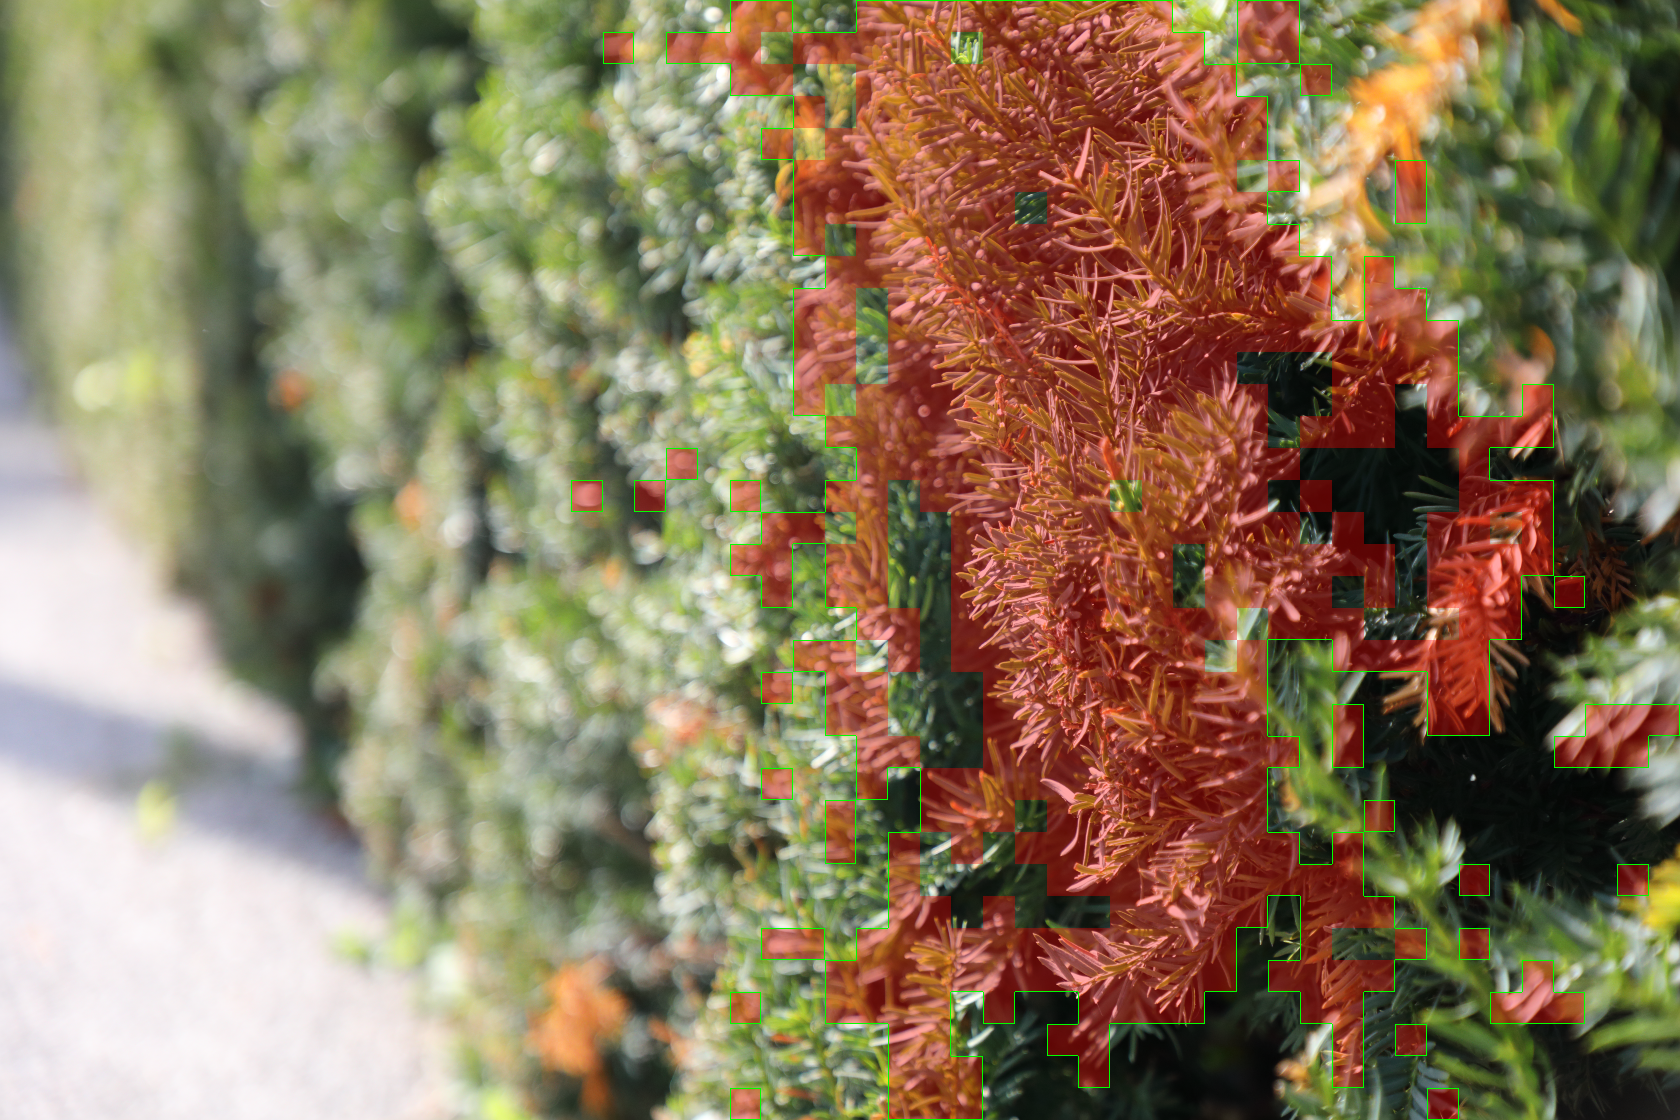
\includegraphics[width=\textwidth]{images/valid_DT_2C.png}
        \caption{Decision Tree}
    \end{subfigure}

    \vspace{0.6em}

    \begin{subfigure}[t]{0.31\textwidth}
        \centering
        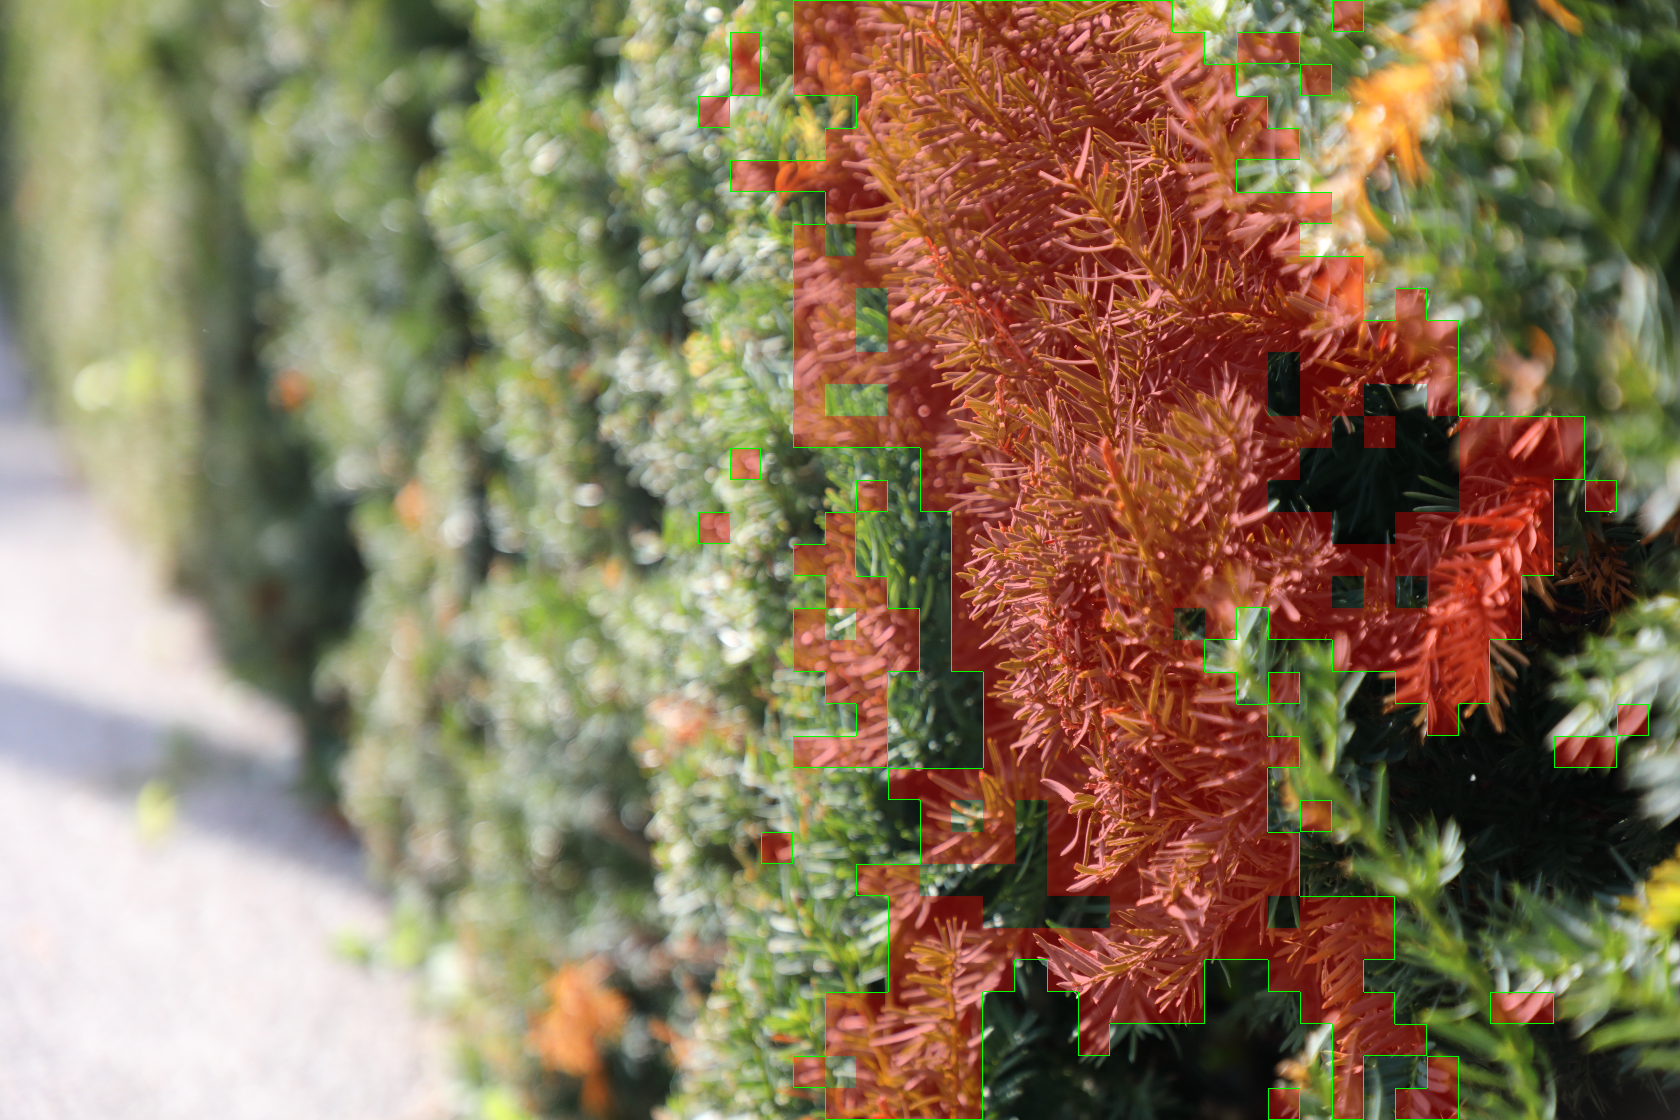
\includegraphics[width=\textwidth]{images/valid1_RF_2C.png}
        \caption{Random Forest}
    \end{subfigure}
    \hfill
    \begin{subfigure}[t]{0.31\textwidth}
        \centering
        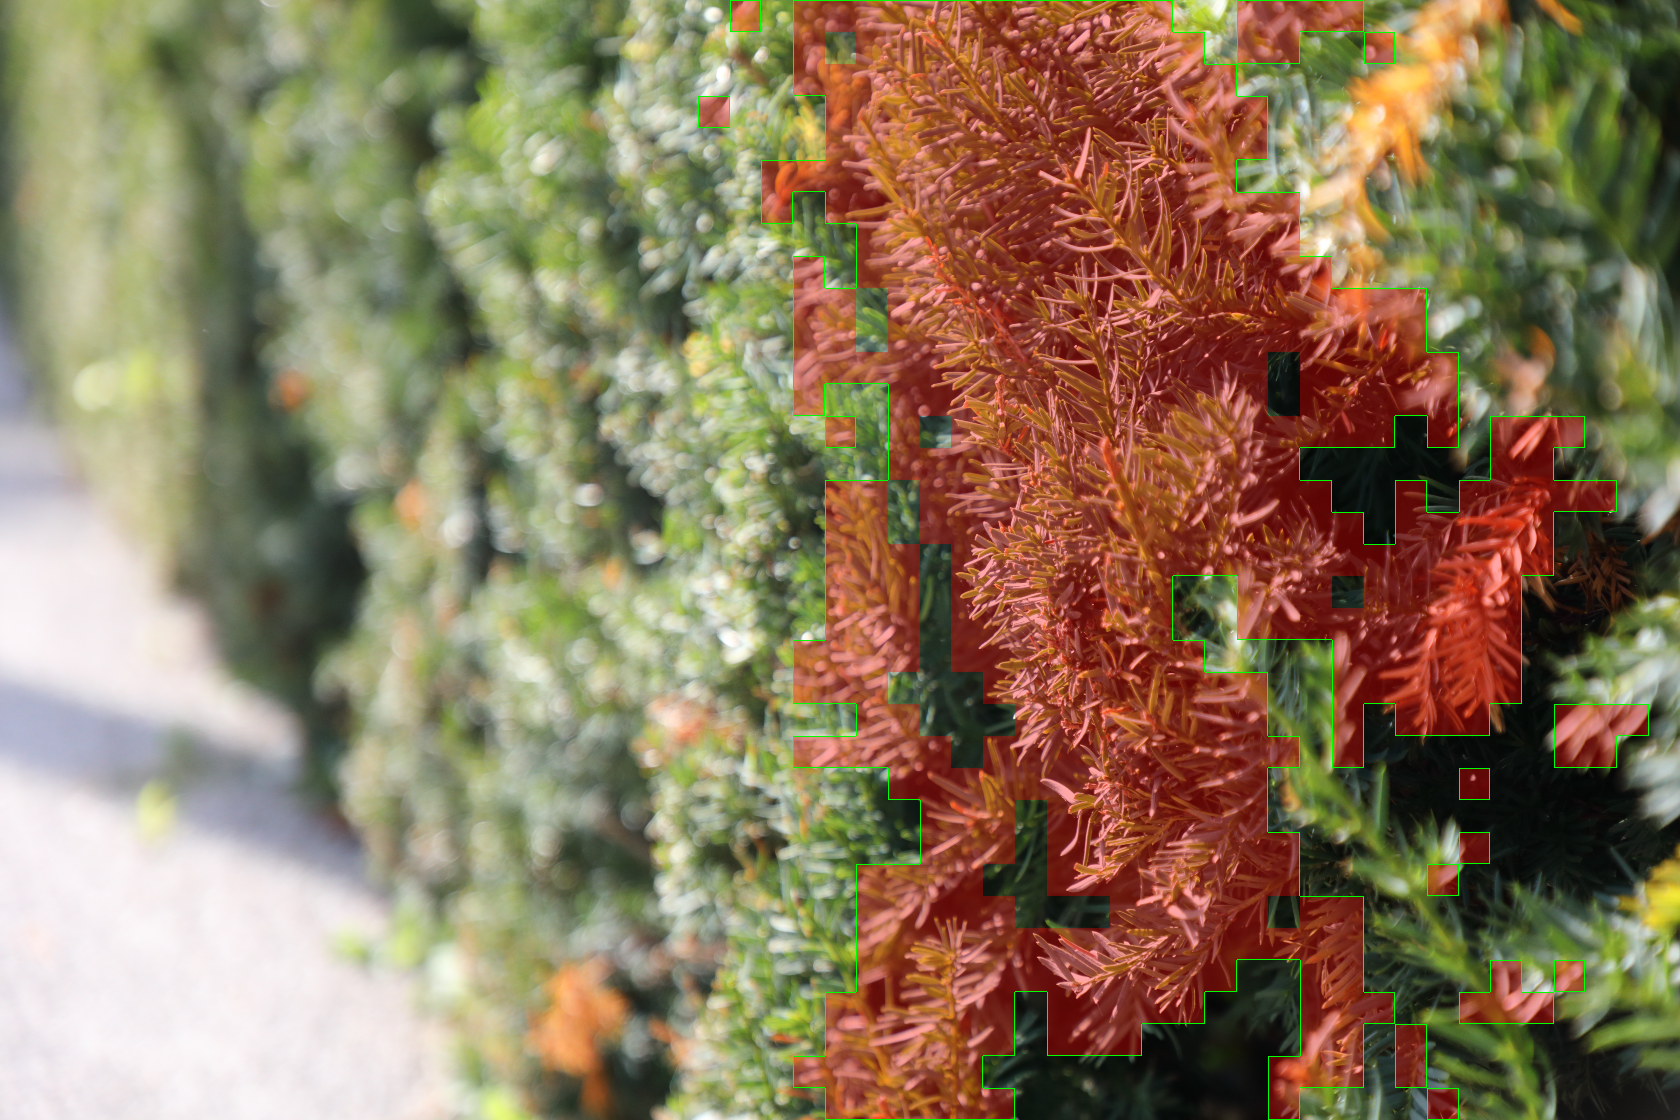
\includegraphics[width=\textwidth]{images/valid1_SVM_2C.png}
        \caption{SVM}
    \end{subfigure}
    \caption{Visualization of manually verified original automatic labels and model predictions under the binary setting}
    \label{fig:valid-2c-compare}
\end{figure}

\par For the three-class task, Fig.~\ref{fig:valid-3c-compare} shows the
corresponding manual verification results. It can be seen that although the
class boundaries are more complex than in the binary task, the main focus
region distribution recovered by each model is still generally consistent with
the original labels. This indicates that although the automatic labeling rule
used in this thesis is approximate, the supervisory signal it generates still
has learnability in terms of spatial distribution. It also indicates that the
later discussion of differences in prediction behavior among different models
is supported jointly by quantitative comparison and manual visual verification.

\begin{figure}[!htbp]
    \centering
    \begin{subfigure}[t]{0.31\textwidth}
        \centering
        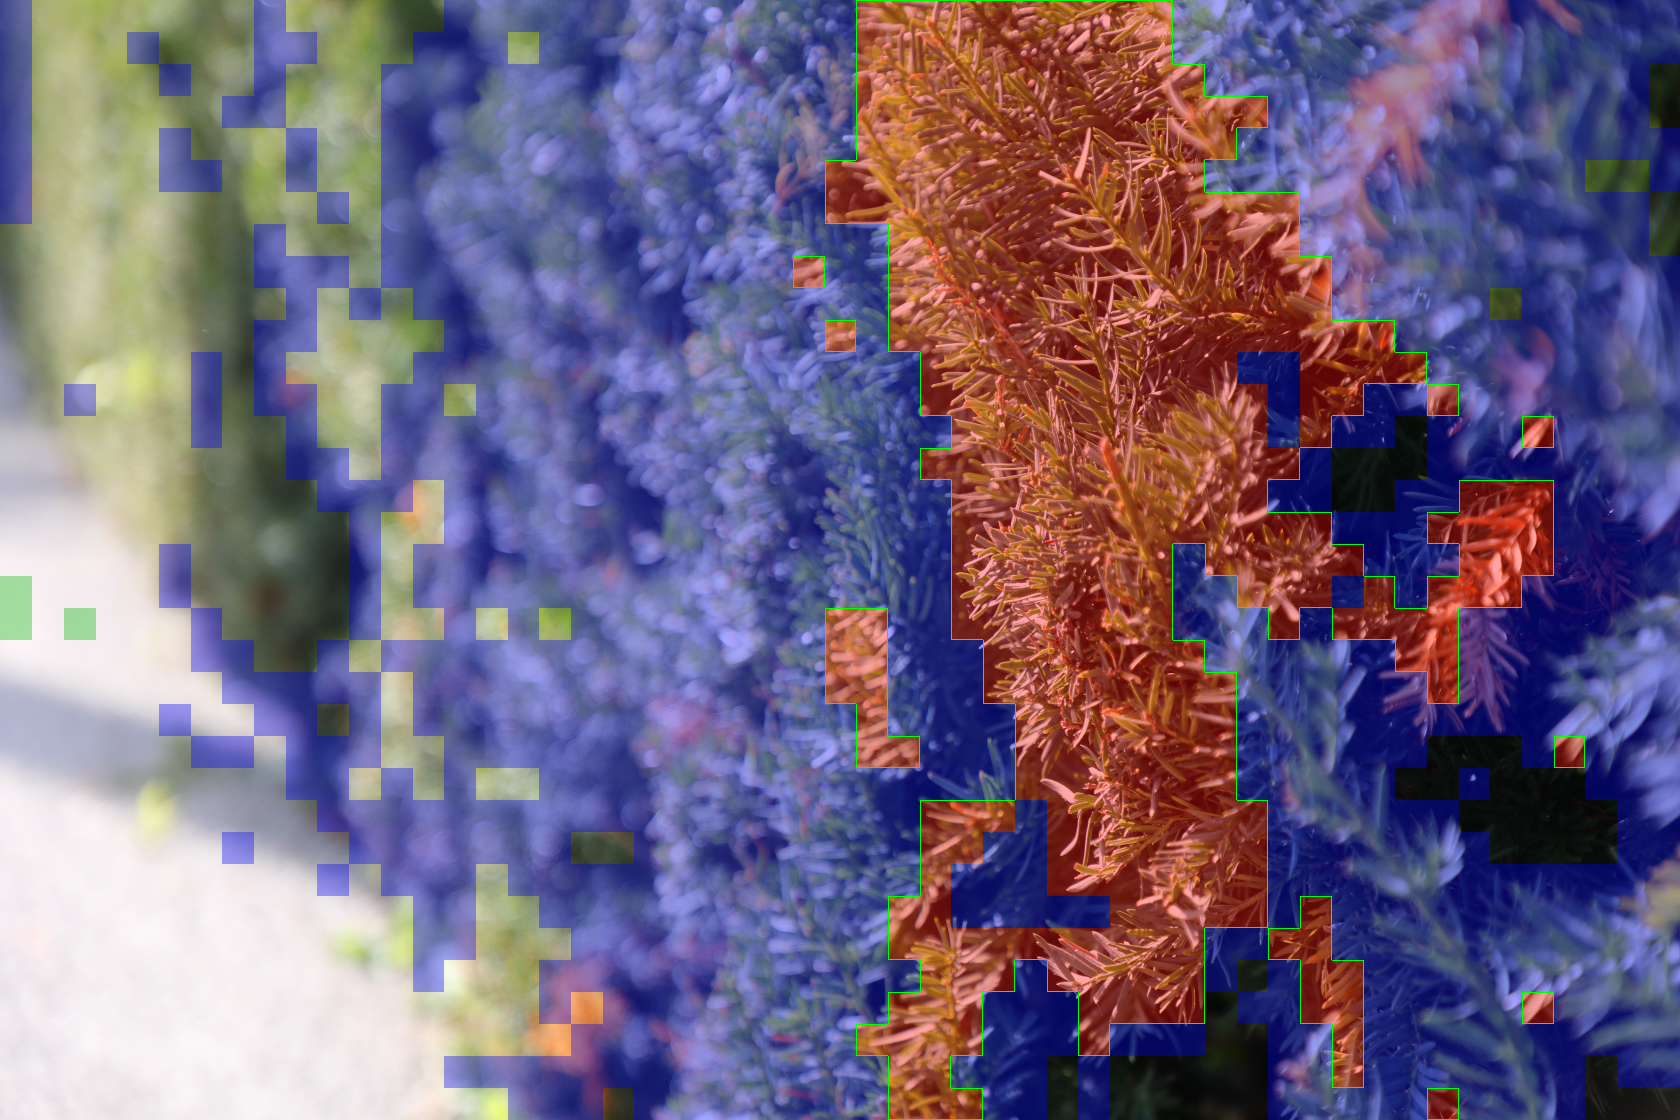
\includegraphics[width=\textwidth]{images/valid1_3C.png}
        \caption{Original auto label}
    \end{subfigure}
    \hfill
    \begin{subfigure}[t]{0.31\textwidth}
        \centering
        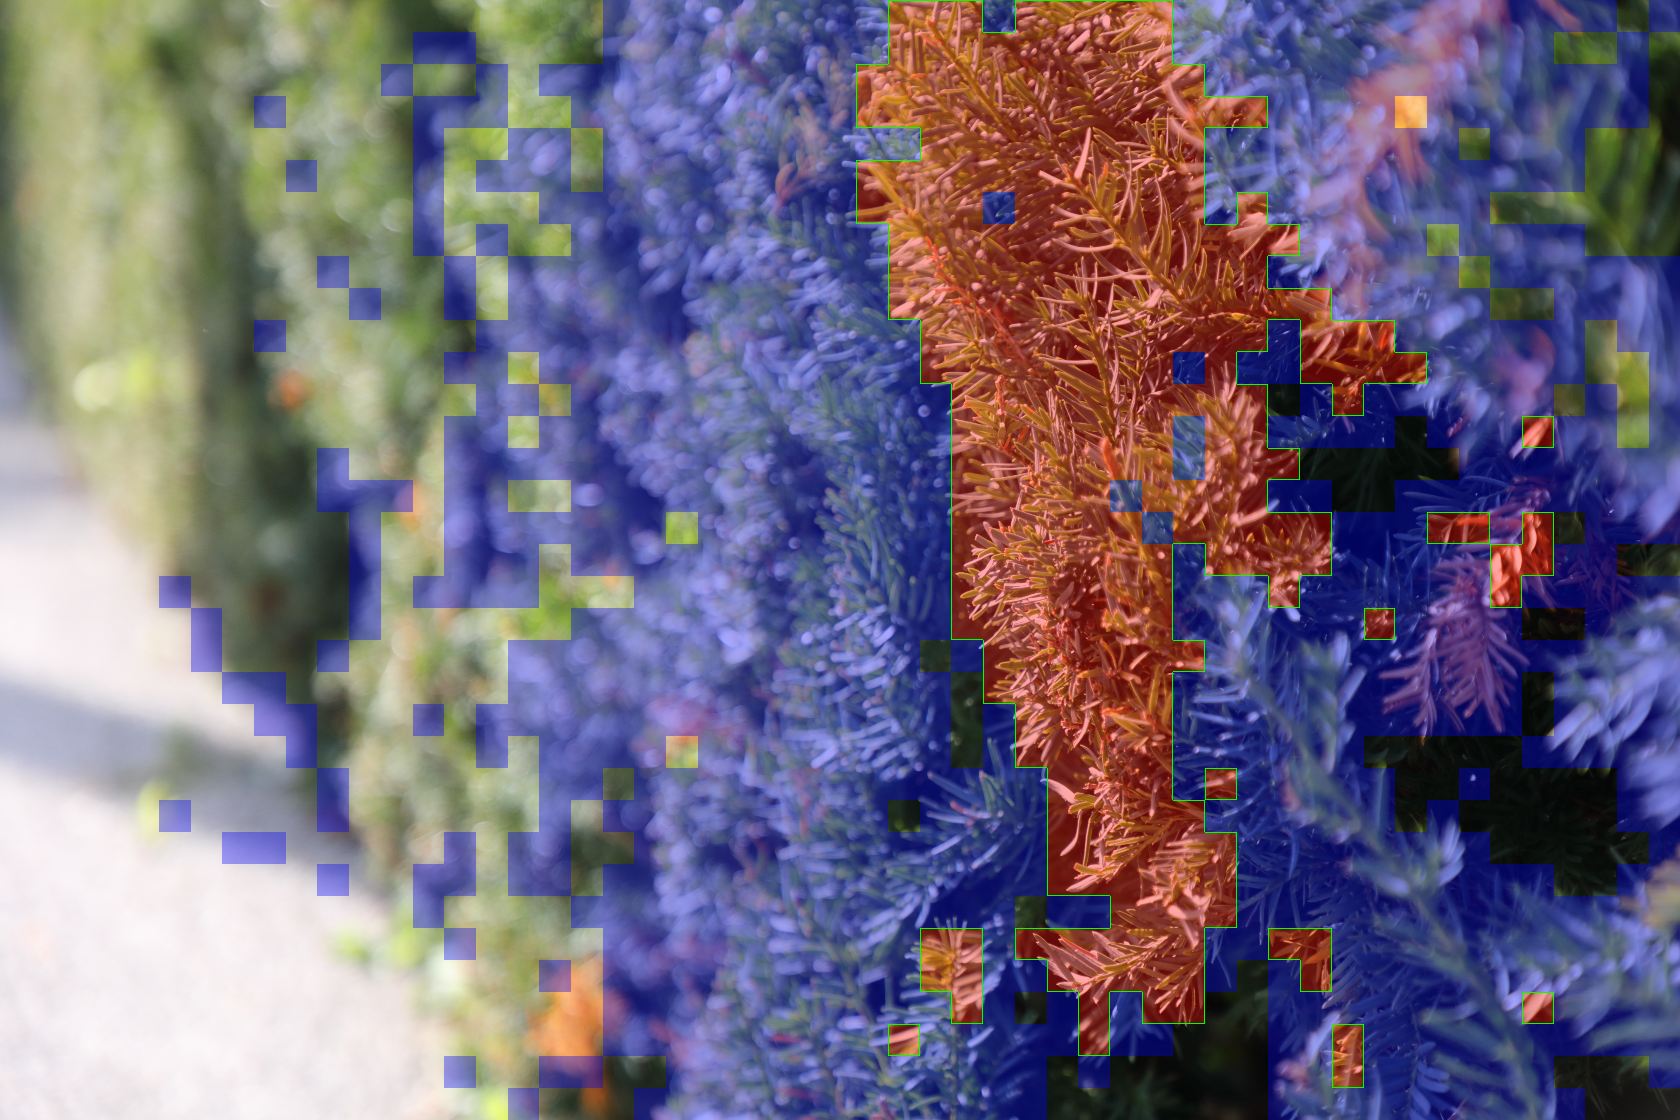
\includegraphics[width=\textwidth]{images/valid1_CNN_3C.png}
        \caption{CNN}
    \end{subfigure}
    \hfill
    \begin{subfigure}[t]{0.31\textwidth}
        \centering
        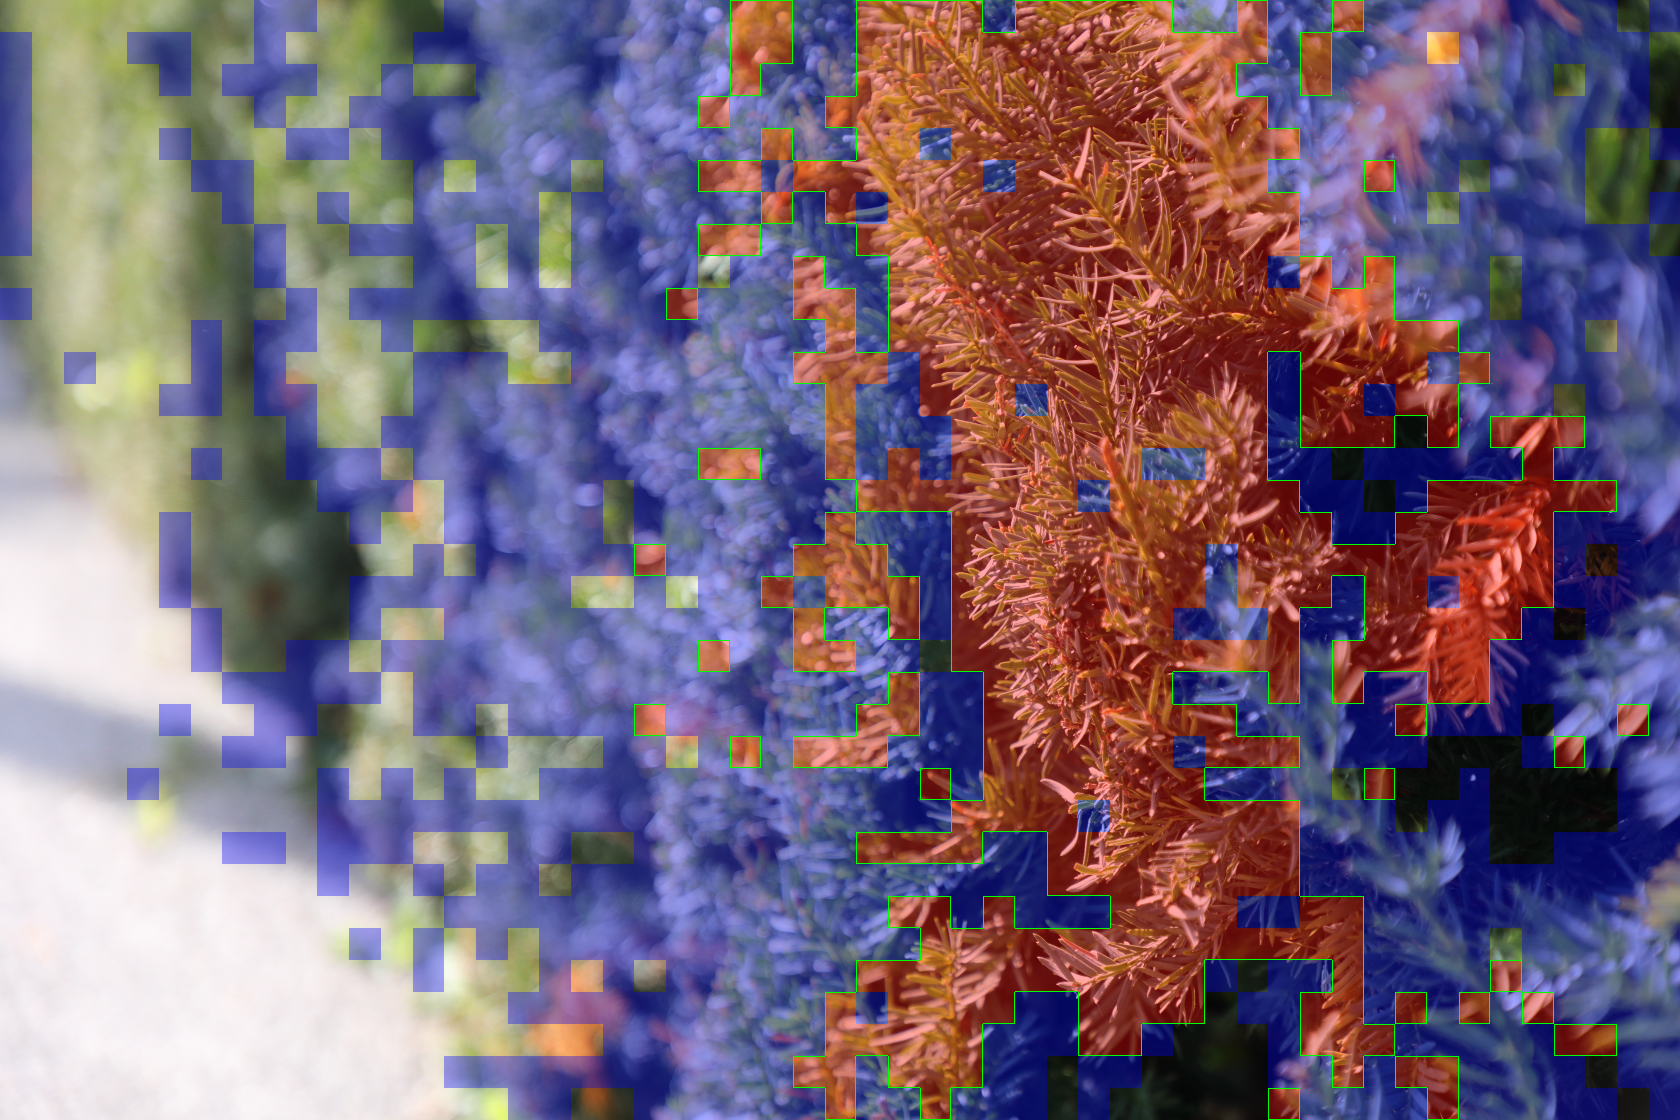
\includegraphics[width=\textwidth]{images/valid1_DT_3C.png}
        \caption{Decision Tree}
    \end{subfigure}

    \vspace{0.6em}

    \begin{subfigure}[t]{0.31\textwidth}
        \centering
        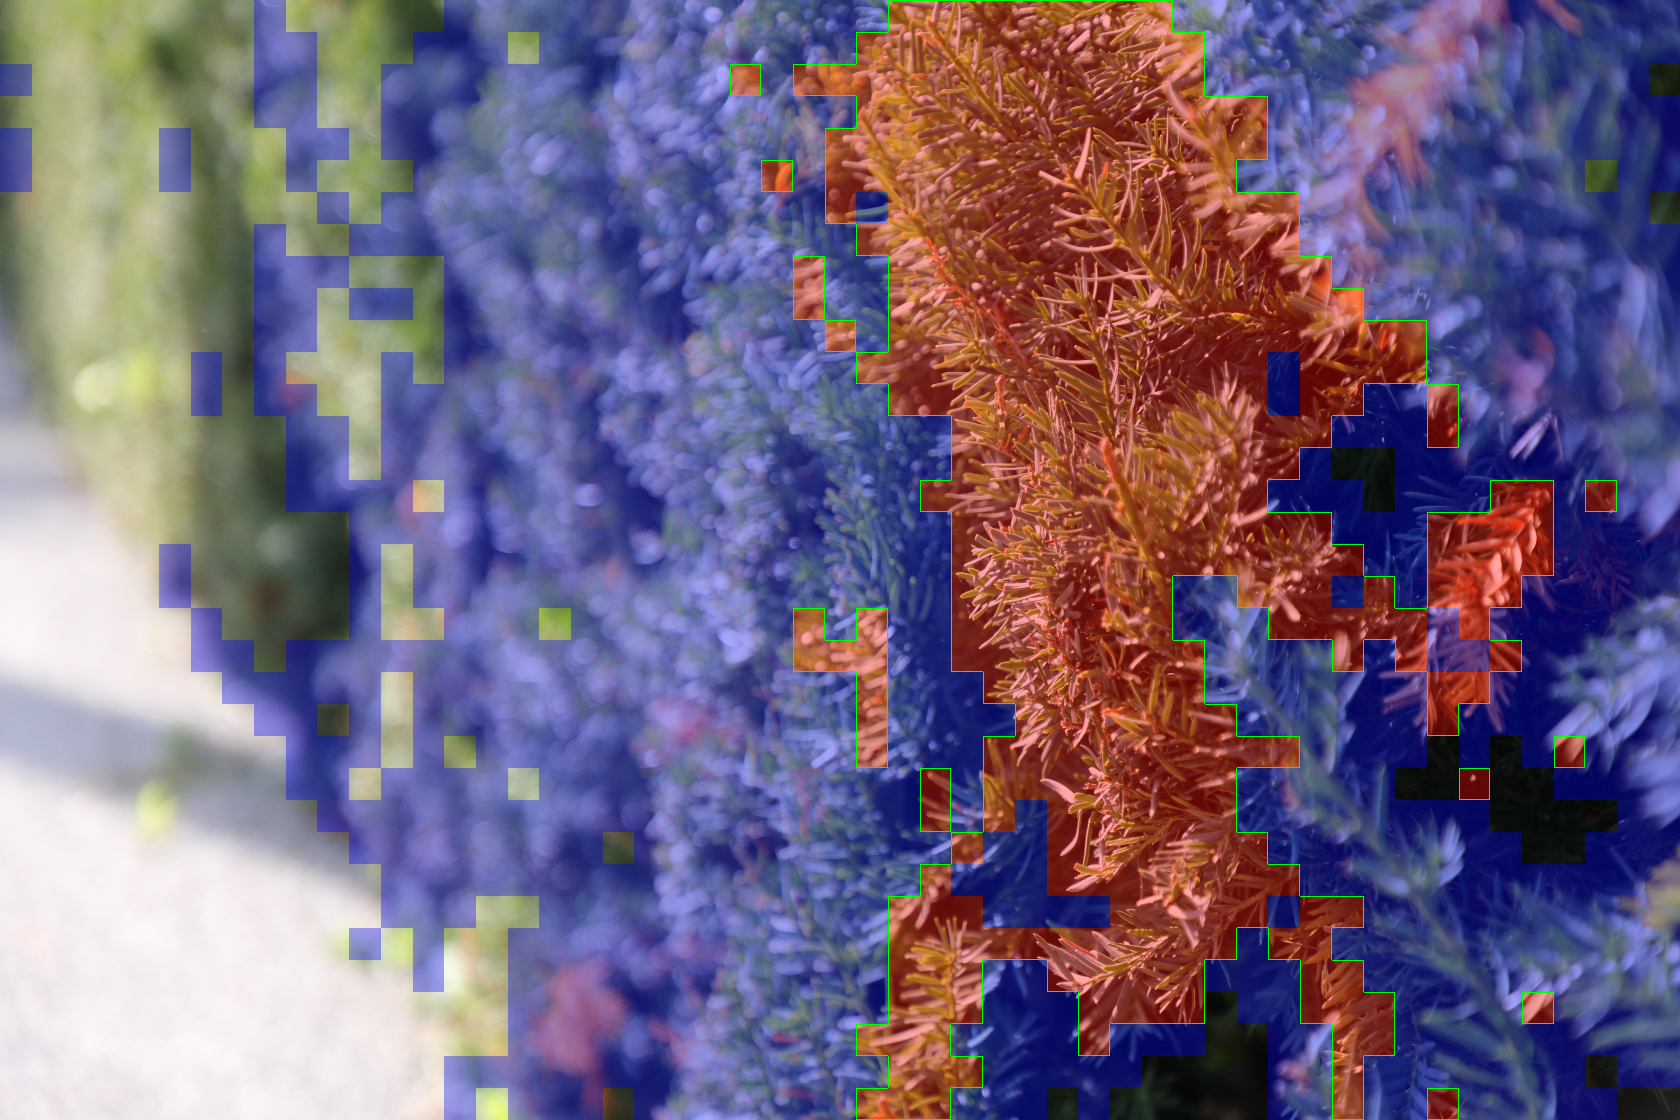
\includegraphics[width=\textwidth]{images/valid1_RF_3C.png}
        \caption{Random Forest}
    \end{subfigure}
    \hfill
    \begin{subfigure}[t]{0.31\textwidth}
        \centering
        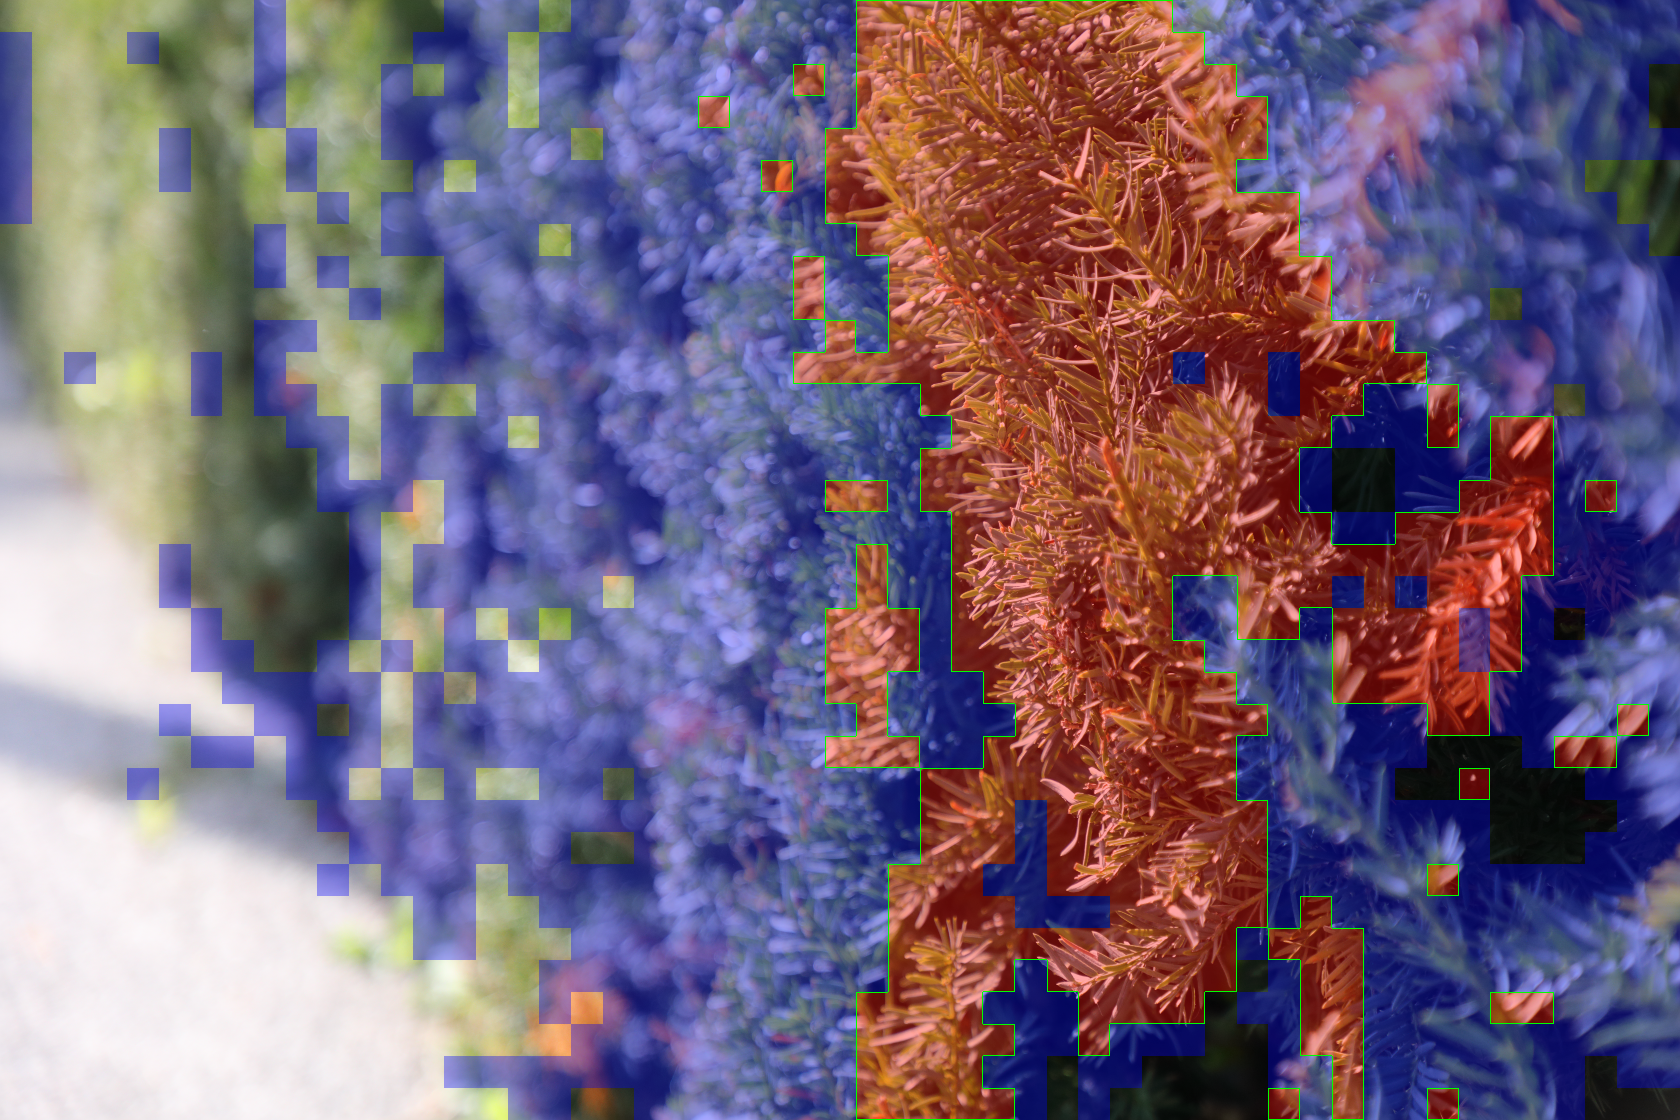
\includegraphics[width=\textwidth]{images/valid1_SVM_3C.png}
        \caption{SVM}
    \end{subfigure}
    \caption{Visualization of manually verified original automatic labels and model predictions under the three-class setting}
    \label{fig:valid-3c-compare}
\end{figure}

\section{Results and Discussion}
\par By combining the pre-experiments, main experiments, sample-size analysis,
manual verification results (Figs.~\ref{fig:valid-2c-compare} and
\ref{fig:valid-3c-compare}), and supplementary experiments in this chapter,
the following overall understanding can be obtained: under the current patch
construction method, PCA representation, and CNN structure setting, the first
factor affecting model performance is task definition, and the second factor is
sample size and training strategy. Overall, the binary task is consistently
easier than the three-class task and can obtain higher and more stable
results. Under the binary setting, the CNN achieves the highest sharp-class
F1-score ($0.84$) and macro F1 ($0.91$) at $100\%$ training samples. Under
the three-class setting, random forest obtains the highest sharp-class F1-score
($0.83$), while the SVM keeps the most stable macro F1, around $0.89$. This
indicates that although separating the intermediate state from the ``non-sharp
class'' is more consistent with the continuous nature of actual focus change,
it also significantly increases the complexity of learning class boundaries,
especially by aggravating the confusion between the sharp class and the
intermediate-state class.

\par The pre-experimental results further verify the rationality of the unified
parameter setting used in the subsequent main experiments. For the classical
models, although a PCA retention ratio of $0.999$ can obtain higher metrics in
some individual experiments, the gain lacks consistency, and the training time
of decision tree and random forest increases clearly. By comparison, a PCA
retention ratio of $0.995$ shows a more balanced performance-cost trade-off in
both binary and three-class tasks. For the CNN, uniformly using $30$ training
epochs reflects the same principle. Compared with $20$ epochs, this setting
can further push loss convergence and bring higher recall and F1-score in the
binary task. When the number of epochs continues to increase to $50$ or $60$,
the training cost grows significantly, but the performance gain is already very
limited. Therefore, the parameter selection in this chapter does not simply
pursue the highest metric in a single experiment, but emphasizes stability,
consistency, and reproducibility across tasks and models.

\par From the main experimental results, different models show relatively clear
role differences. In both tasks, decision tree can serve as a low-cost
baseline, but as training samples increase, its performance quickly enters a
plateau, which indicates that its ability to represent complex class
boundaries is relatively limited. Random forest is the most aggressive
traditional model in detecting the sharp class and can usually obtain high
recall. It also achieves the highest sharp-class F1-score in the three-class
task. At the same time, however, its precision decreases as sample size
increases, showing a relatively obvious precision-recall trade-off. The SVM,
in contrast, shows the most stable overall generalization ability. In the
binary task, it maintains nearly fixed high recall ($0.97$) and stable
F1-score at relatively low training cost. In the three-class task, it
continuously keeps the most stable macro F1, which indicates that the
combination of Nystr\"{o}m kernel mapping and PCA features is well suited to
the current task. The main advantage of the CNN lies in the binary task, where
it achieves the highest sharp-class F1-score by relying on extremely high
precision. However, under the three-class setting, the default training
configuration makes its judgment on the sharp class too conservative, thus
limiting recall improvement. This indicates that the potential advantage of
deep models does not automatically appear as task complexity increases, but
still depends on more suitable training mechanisms and decision strategies.

\par The sample-size analysis indicates that although increasing training data
can generally bring some benefit, it is not the decisive factor for improving
the performance of the current system. In the scan from $20\%$ to $100\%$
samples, the metric changes of most models mainly appear as slight improvement
or small fluctuation, while training time increases almost monotonically with
the sample ratio. This indicates that under the current experimental
framework, the marginal benefit of sample expansion is relatively limited, and
the model structure, feature representation, and decision-threshold setting
affect final performance more directly. The supplementary experiments further
support this judgment. For the binary CNN, enabling the weighted sampler alone
is not better than the main experimental configuration, and the factor that
really changes the result is later threshold calibration. For the three-class
CNN, by contrast, the weighted sampler significantly improves sharp-class
recall and F1-score. This indicates that when the intermediate-state class is
introduced into the task, the learning pressure on the minority class becomes a
more important factor limiting performance. Therefore, the performance
bottlenecks are not the same under different task settings, and the training
strategy should not be copied mechanically, but instead designed according to
the specific problem.

\par Based on the above analysis, this thesis considers that future system
design can choose models according to the task objective, rather than pursuing
an abstract single ``best model''. If the goal is to obtain high overall
sharp-class recognition ability in the binary task, the CNN is a solution worth
prioritizing. If high recall and low training cost are emphasized more, the
SVM may have higher practical cost-effectiveness. For the three-class task, if
sharp-class detection effect is the priority, random forest can be considered
first. If overall class balance and result stability are more important, the
SVM may be more suitable. As for the CNN, if it is still taken as the key
model for the three-class scenario in future work, then the weighted sampler,
threshold calibration, and stronger data augmentation should be regarded as
priority directions for improvement, rather than simply continuing to enlarge
sample size or training epochs. Overall, the results in this chapter show that
the core problem in local focus detection is not only whether the sample size
is large enough. More importantly, it is how to establish a more reasonable
modeling and training scheme under class imbalance, ambiguous class boundaries,
and computational-cost constraints. This understanding also provides a direct
basis for the system implementation and method improvement in the next chapter.
